% WCTR / Transportation Research Procedia manuscript
\documentclass[3p,times,procedia]{elsarticle}
\flushbottom

\usepackage{ecrc}
\usepackage{fancyhdr}
\pagestyle{fancy}
\fancyhf{}
\fancyfoot[R]{\thepage}
\renewcommand{\headrulewidth}{0pt}
\renewcommand{\footrulewidth}{0pt}

\volume{00}
\firstpage{1}
\journalname{Transportation Research Procedia}
\runauth{Zaman, Tomal, Chayan, Pandit, Cirillo}
\jid{trpro}

\usepackage{amssymb}
\usepackage{amsmath}
\usepackage{graphicx}
\usepackage{booktabs}
\usepackage{float}
\usepackage[figuresright]{rotating}
\usepackage{caption}
\usepackage{siunitx}
\usepackage{array}
\usepackage{tabularx}
\usepackage{longtable}
\captionsetup[table]{skip=8pt}
\graphicspath{{latex-figures/}}
\usepackage[bookmarks=false,colorlinks,linkcolor=blue,citecolor=blue,urlcolor=blue]{hyperref}

\biboptions{numbers,sort&compress}

\DeclareMathOperator{\TVD}{TVD}
\DeclareMathOperator{\JS}{JS}
\DeclareMathOperator{\KL}{KL}

\begin{document}
\pagenumbering{arabic}
\begin{frontmatter}

\dochead{World Conference on Transport Research - Toulouse 6-10 July 2026}

\title{Contrastive VAE-Generated Trip Data from Travel Surveys: Population-Scale Synthesis and Screenline Count Validation}

\author[a]{Raziq Zaman}
\ead{raziq@umd.edu}
\author[a]{Raas Sarker Tomal}
\ead{rtomal@umd.edu}
\author[a]{Md Mahmudul Huque Chayan}
\ead{mchayan@umd.edu}
\author[a]{Darshan Pandit}
\ead{dmpandit@umd.edu}
\author[a]{Cinzia Cirillo}
\ead{ccirillo@umd.edu}

\address[a]{Department of Civil and Environmental Engineering, University of Maryland}

\begin{abstract}
Household travel surveys contain the behavioral richness needed for disaggregate travel-demand modeling, but their samples are sparse relative to the population, especially in high-cardinality origin-destination and activity-time spaces. This paper develops and evaluates a contrastive mixed-tabular variational autoencoder (VAE) for synthesizing population-scale trip records from travel-survey microdata. The implemented experiment, \texttt{paper\_wctr\_1m\_vae\_sweep}, uses \num{110926} transformed survey trip records with \num{44} synthesizable features, excludes the survey expansion weight from generated outputs, and uses the sum of expansion weights, \num{19287211.91}, as the population target. Each compared method is capped at \num{1000000} generated rows and scaled back to the population target for count validation. Four methods are evaluated: weighted bootstrap resampling, a weighted Chow-Liu-style Bayesian network, a noncontrastive mixed-tabular VAE, and an otherwise identical contrastive VAE.

The contrastive VAE embeds categorical trip fields, standardizes numeric fields, and optimizes a weighted reconstruction-plus-KL objective augmented with an InfoNCE representation regularizer. Positive views lightly perturb non-key attributes, while marginal negatives corrupt categorical values and shuffle numeric values. Internal validation compares weighted survey and synthetic one-way marginals, selected two-way cross-marginals, exact-row copying, duplicate rates, invalid-category rates, and novel origin-destination support. External validation uses a two-prong tract-boundary screenline proxy: dense annual-average screenline counts from MDOT SHA AADT/AAWDT stations and sparse hourly counts from FHWA TMAS stations scaled by annual station share. Results show that bootstrap resampling is strongest on internal marginals but copies all records by design. The contrastive VAE has zero exact-row copy rate, produces \num{395542} unique directed origin-destination tract pairs in a one-million-row sample compared with \num{58925} in the survey input, and improves cross-marginal total variation from 0.2556 to 0.2265 relative to the noncontrastive VAE. In external validation, learned generators substantially reduce hourly TMAS RMSE relative to weighted bootstrap; the contrastive VAE has the lowest hourly RMSE, while annual-average screenline totals remain difficult and reveal the limits of current centroid-line assignment. The contribution is therefore not a claim of fully calibrated traffic assignment, but a reproducible synthesis-and-validation framework for judging whether generative trip records preserve marginal, joint, privacy, spatial-support, and independent count-plausibility properties simultaneously.
\end{abstract}

\begin{keyword}
Synthetic trip data; Variational autoencoder; Contrastive learning; Household travel survey; Population synthesis; Traffic count validation; Screenline validation
\end{keyword}

\end{frontmatter}

\section*{Highlights}
\begin{itemize}
    \item A contrastive mixed-tabular VAE synthesizes weighted travel-survey trip records without generating the expansion-weight field.
    \item Internal validation separates one-way fit, dependence fit, exact copying, duplicate generation, invalid categories, and novel origin-destination support.
    \item External validation uses independent MDOT annual-average traffic counts and FHWA TMAS hourly counts through a transparent tract-boundary screenline proxy.
    \item The contrastive regularizer improves VAE cross-marginal fit and numeric distribution fit while preserving zero exact-row copy rate.
\end{itemize}

\newpage

\section{Introduction}
Activity-based and agent-based transport models require detailed trip records: who travels, when they leave, how long they travel, why they travel, where they begin, and where they end. Platforms such as MATSim make this demand explicit because the simulated system is built from individual agents and their plans \cite{horni2016matsim}. Household travel surveys provide exactly this behavioral detail, but they observe only a small fraction of the population. Direct survey expansion can reproduce weighted marginal totals, but it also repeats observed records and leaves sparse support in the high-dimensional spaces where planning models need plausible combinations of activity purpose, mode, time, vehicle, household attributes, and tract-to-tract movement. This tension is old in transportation modeling: the analyst needs population-scale microdata, but the most informative source is a limited survey sample \cite{beckman1996creating,farooq2013simulation}.

Deep generative models offer a complementary route. Rather than only reweighting observed households or trips, they can learn a high-dimensional joint distribution and sample new records from it. Variational autoencoders (VAEs) are especially attractive because their latent prior gives a direct sampling mechanism \cite{kingma2014autoencoding}. Yet trip data are not image data. They are mixed tabular records with unordered categorical fields, integer-valued ordinal fields, continuous distances, survey weights, high-cardinality tract identifiers, and sparse but meaningful origin-destination combinations. A credible generative trip model must respect these data contracts and must be evaluated beyond marginal overlap.

This paper reports the current experiment implemented in the repository run \texttt{outputs/runs/paper\_wctr\_1m\_vae\_sweep}. The research question is practical: can a contrastive VAE generate trip records that preserve weighted survey distributions, improve joint structure relative to an identical noncontrastive VAE, avoid exact row copying, expand plausible origin-destination support, and produce reasonable aggregate traffic-count patterns when tested against independent screenline data?

The answer is deliberately nuanced. Weighted bootstrap resampling remains the strongest internal marginal baseline, but it copies survey records by construction. A Bayesian network baseline preserves one-way distributions well but is less expressive for selected two-way behavioral dependencies. The contrastive VAE is weaker than copying on one-way marginals, but it generates many more origin-destination pairs, avoids exact copying, and improves cross-marginal fidelity relative to the noncontrastive VAE. External traffic-count validation is mixed: learned generators reduce hourly TMAS RMSE relative to bootstrap, but annual screenline totals remain difficult under a centroid-line tract-crossing proxy. The methodological contribution is therefore a rigorous generative trip synthesis and validation harness, not a claim that the VAE alone solves population synthesis or traffic assignment.

\section{Literature Review}\label{sec:literature}
\subsection{Synthetic Populations and Survey Expansion}
Synthetic population generation is a foundational input to disaggregate transport modeling. Early transportation microsimulation systems such as TRANSIMS used synthetic baseline populations to create agent-level demand inputs from census and survey data \cite{beckman1996creating}. Iterative proportional fitting, iterative proportional updating, combinatorial optimization, and simulation-based synthesis have remained important because they can match external control totals and preserve interpretable constraints \cite{farooq2013simulation}. Open-data pipelines for activity-based modeling, including the Paris and Ile-de-France synthetic population and travel-demand system, show how public census, land-use, and transport data can be assembled into complete agent-based demand inputs \cite{horl2021synthetic}. These methods are strong when control totals are available and the target representation is well specified. They are weaker when the analyst asks a sample to support many high-cardinality combinations for which no direct controls are available.

Travel-survey trip synthesis has a related but distinct challenge. A trip table is not only a population table; it couples household, person, vehicle, activity, time, and origin-destination attributes in one behavioral record. Expansion weights provide scale, but scale is not the same as joint support. Repeated weighted resampling can preserve empirical weighted distributions, but repeated records are problematic for privacy diagnostics, uncertainty representation, and downstream agent diversity. This paper therefore treats survey weights as population expansion and training weights, not as variables to be generated.

\subsection{Deep Generative Models for Tabular and Transport Data}
VAEs introduced amortized variational inference with a differentiable reparameterization trick, making it practical to learn latent-variable generative models with neural encoders and decoders \cite{kingma2014autoencoding,rezende2014stochastic}. Beta-VAE variants show that weighting the KL term can change the tradeoff between reconstruction fidelity and latent regularization \cite{higgins2017beta}. For tabular data, the key issue is mixed type structure. Continuous variables and unordered categories should not be forced into a single ordinal reconstruction loss. CTGAN and TVAE work highlighted the need for column-specific treatment of discrete and continuous tabular variables and for evaluating tabular generators against statistical baselines \cite{xu2019modeling}.

In transportation, Borysov, Rich, and Pereira demonstrated that VAEs can scale population synthesis to high-dimensional travel-survey settings and can address sampling zeros better than pure frequency-table methods \cite{borysov2019scalable}. Garrido and coauthors sharpened this point by distinguishing sampling zeros from structural zeros in rare feature-combination prediction \cite{garrido2020prediction}. Kim and Bansal similarly argued that deep generative models must balance diversity with feasibility when synthesizing populations for activity-based models \cite{kim2023deep}. These studies motivate the present paper's emphasis on novel origin-destination support and validity diagnostics: a useful generator should not merely copy observed records, but novelty is valuable only if the generated records remain behaviorally and spatially plausible.

\subsection{Contrastive Learning for Tabular Representation}
Contrastive learning trains representations by pulling together related views and pushing apart unrelated or corrupted views. Contrastive predictive coding introduced a probabilistic contrastive loss using negative sampling, often referred to through the InfoNCE objective \cite{oord2018representation}. In tabular domains, SCARF showed that random feature corruption can create useful self-supervised views for tabular representation learning \cite{bahri2022scarf}. The contrastive VAE in this paper uses the same broad idea but with trip-specific constraints: positives are light perturbations that avoid protected origin, destination, and timing fields, while negatives are marginally corrupted records. The contrastive term is not a separate generator; it regularizes the VAE encoder so that latent representations are less brittle to small non-key perturbations and more discriminative against implausible marginal recombinations.

\subsection{Validation Beyond Marginals}
Marginal similarity is necessary but not sufficient. A model can match each column and still fail on joint dependencies, spatial support, copying risk, or external traffic plausibility. The Bayesian-network baseline in this paper follows the information-theoretic tradition of Chow and Liu, where a maximum mutual-information tree approximates a multivariate discrete distribution \cite{chow1968approximating}. That baseline is interpretable and strong on simple distributions, but a tree cannot represent all higher-order interactions in a trip table.

Privacy diagnostics are similarly essential. Exact row copy rate and duplicate rate are not formal privacy guarantees, and this paper does not claim differential privacy in the sense of Dwork and coauthors \cite{dwork2006calibrating}. They are nevertheless important utility-risk diagnostics because synthetic data can otherwise appear accurate by memorizing source records. Recent synthetic-data privacy critiques caution that synthetic release should not be confused with anonymization unless the privacy mechanism is explicit and auditable \cite{stadler2022synthetic}. The present work therefore reports copying and invalid-category diagnostics transparently.

Finally, transport validation should test generated demand against data not used for training. Traffic monitoring programs provide such external signals. FHWA's traffic monitoring program receives continuous count data from state agencies and publishes Traffic Monitoring Analysis System (TMAS) data \cite{fhwa_tmas_data}. MDOT SHA's AADT layer provides Maryland traffic-count station geometry and annual-average count fields for thousands of locations \cite{mdot_aadt_2019}. These data do not make the present screenline proxy a full network assignment model, but they provide a valuable independent check: synthetic trips that look good internally should also produce plausible aggregate crossings when projected through a consistent spatial proxy.

\section{Data and Experimental Design}\label{sec:data}
\subsection{Survey Input and Feature Contract}
The implemented paper run uses the transformed survey file \texttt{05\_transformed\_survey.csv}, a long-format trip table derived from the Maryland statewide and regional travel-survey inputs \cite{bmc2019mts,mwcog2018rts}. The final modeling file contains \num{110926} rows and \num{45} columns, including the survey expansion weight \texttt{weight}. The synthesis schema excludes \texttt{weight}, leaving \num{44} generated features: \num{26} categorical fields, \num{17} ordinal integer fields, and one continuous field. Origin, destination, home, and work tract FIPS codes are cleaned as 11-digit strings; the \texttt{year} field is vehicle model year, not survey trip year.

The sum of survey expansion weights is \num{19287211.91}. The run therefore defines the population target as \num{19287212} trips, but each method is capped at \num{1000000} generated rows for tractable file size and validation runtime. Count validation multiplies each method's synthetic crossings by the recorded sample expansion factor, \num{19.287212}. Table~\ref{tab:data-contract} summarizes the implemented data contract.

\begin{table}[H]
\centering
\caption{Implemented survey and synthesis data contract for \texttt{paper\_wctr\_1m\_vae\_sweep}.}
\label{tab:data-contract}
\footnotesize
\begin{tabularx}{\linewidth}{lX}
\toprule
\textbf{Item} & \textbf{Implemented value} \\
\midrule
Input file & \texttt{05\_transformed\_survey.csv}. \\
Survey rows & \num{110926} trip records. \\
Columns & \num{45} total columns, including \texttt{weight}. \\
Synthesized features & \num{44} features; \texttt{weight} is excluded from every synthetic output. \\
Categorical features & \num{26} fields with \num{11010} learned category levels; largest vocabularies are destination tract, origin tract, home tract, work tract, and vehicle. \\
Numeric features & \num{18} numeric fields: \num{17} ordinal integer fields and one continuous distance field. \\
Survey expansion target & \num{19287211.91} weighted trips, rounded to \num{19287212}. \\
Per-method generated rows & \num{1000000} rows, with count-validation expansion factor \num{19.287212}. \\
Observed tract support & \num{2649} unique origin tracts, \num{2764} unique destination tracts, and \num{58925} observed directed origin-destination tract pairs. \\
Survey period for count validation & October 1, 2017 through July 31, 2019; dates are reconstructed from \texttt{tdate\_week} and \texttt{tdate\_dow}. \\
\bottomrule
\end{tabularx}
\end{table}

\subsection{Compared Methods}
The run compares four methods under the same input table, schema, seed, one-million-row cap, and validation suite.

\textbf{Weighted bootstrap.} Rows are resampled with replacement using probabilities proportional to nonnegative survey weights. This is a strong internal-distribution baseline because it directly reuses empirical records. It is also expected to have high exact-row copy rate.

\textbf{Bayesian network.} Numeric fields are discretized into at most \num{16} bins. Weighted pairwise mutual information is estimated across features, and a maximum-spanning-tree dependency structure is fit in the spirit of Chow-Liu trees \cite{chow1968approximating}. The model samples from the weighted root marginal and weighted conditional probability tables with additive smoothing of 1.0. Numeric values are decoded by sampling observed training values from the selected bin. The paper run caps Bayesian-network fit and sampling at \num{3600} seconds and samples in chunks of \num{50000} rows.

\textbf{Noncontrastive VAE.} This ablation uses the same mixed-tabular VAE architecture as the contrastive model but sets the contrastive coefficient to zero. It isolates the effect of the representation regularizer.

\textbf{Contrastive VAE.} The proposed method adds a contrastive encoder regularizer to the same VAE architecture and training process. Its configuration is summarized in Table~\ref{tab:vae-config}.

\begin{figure}[H]
\centering
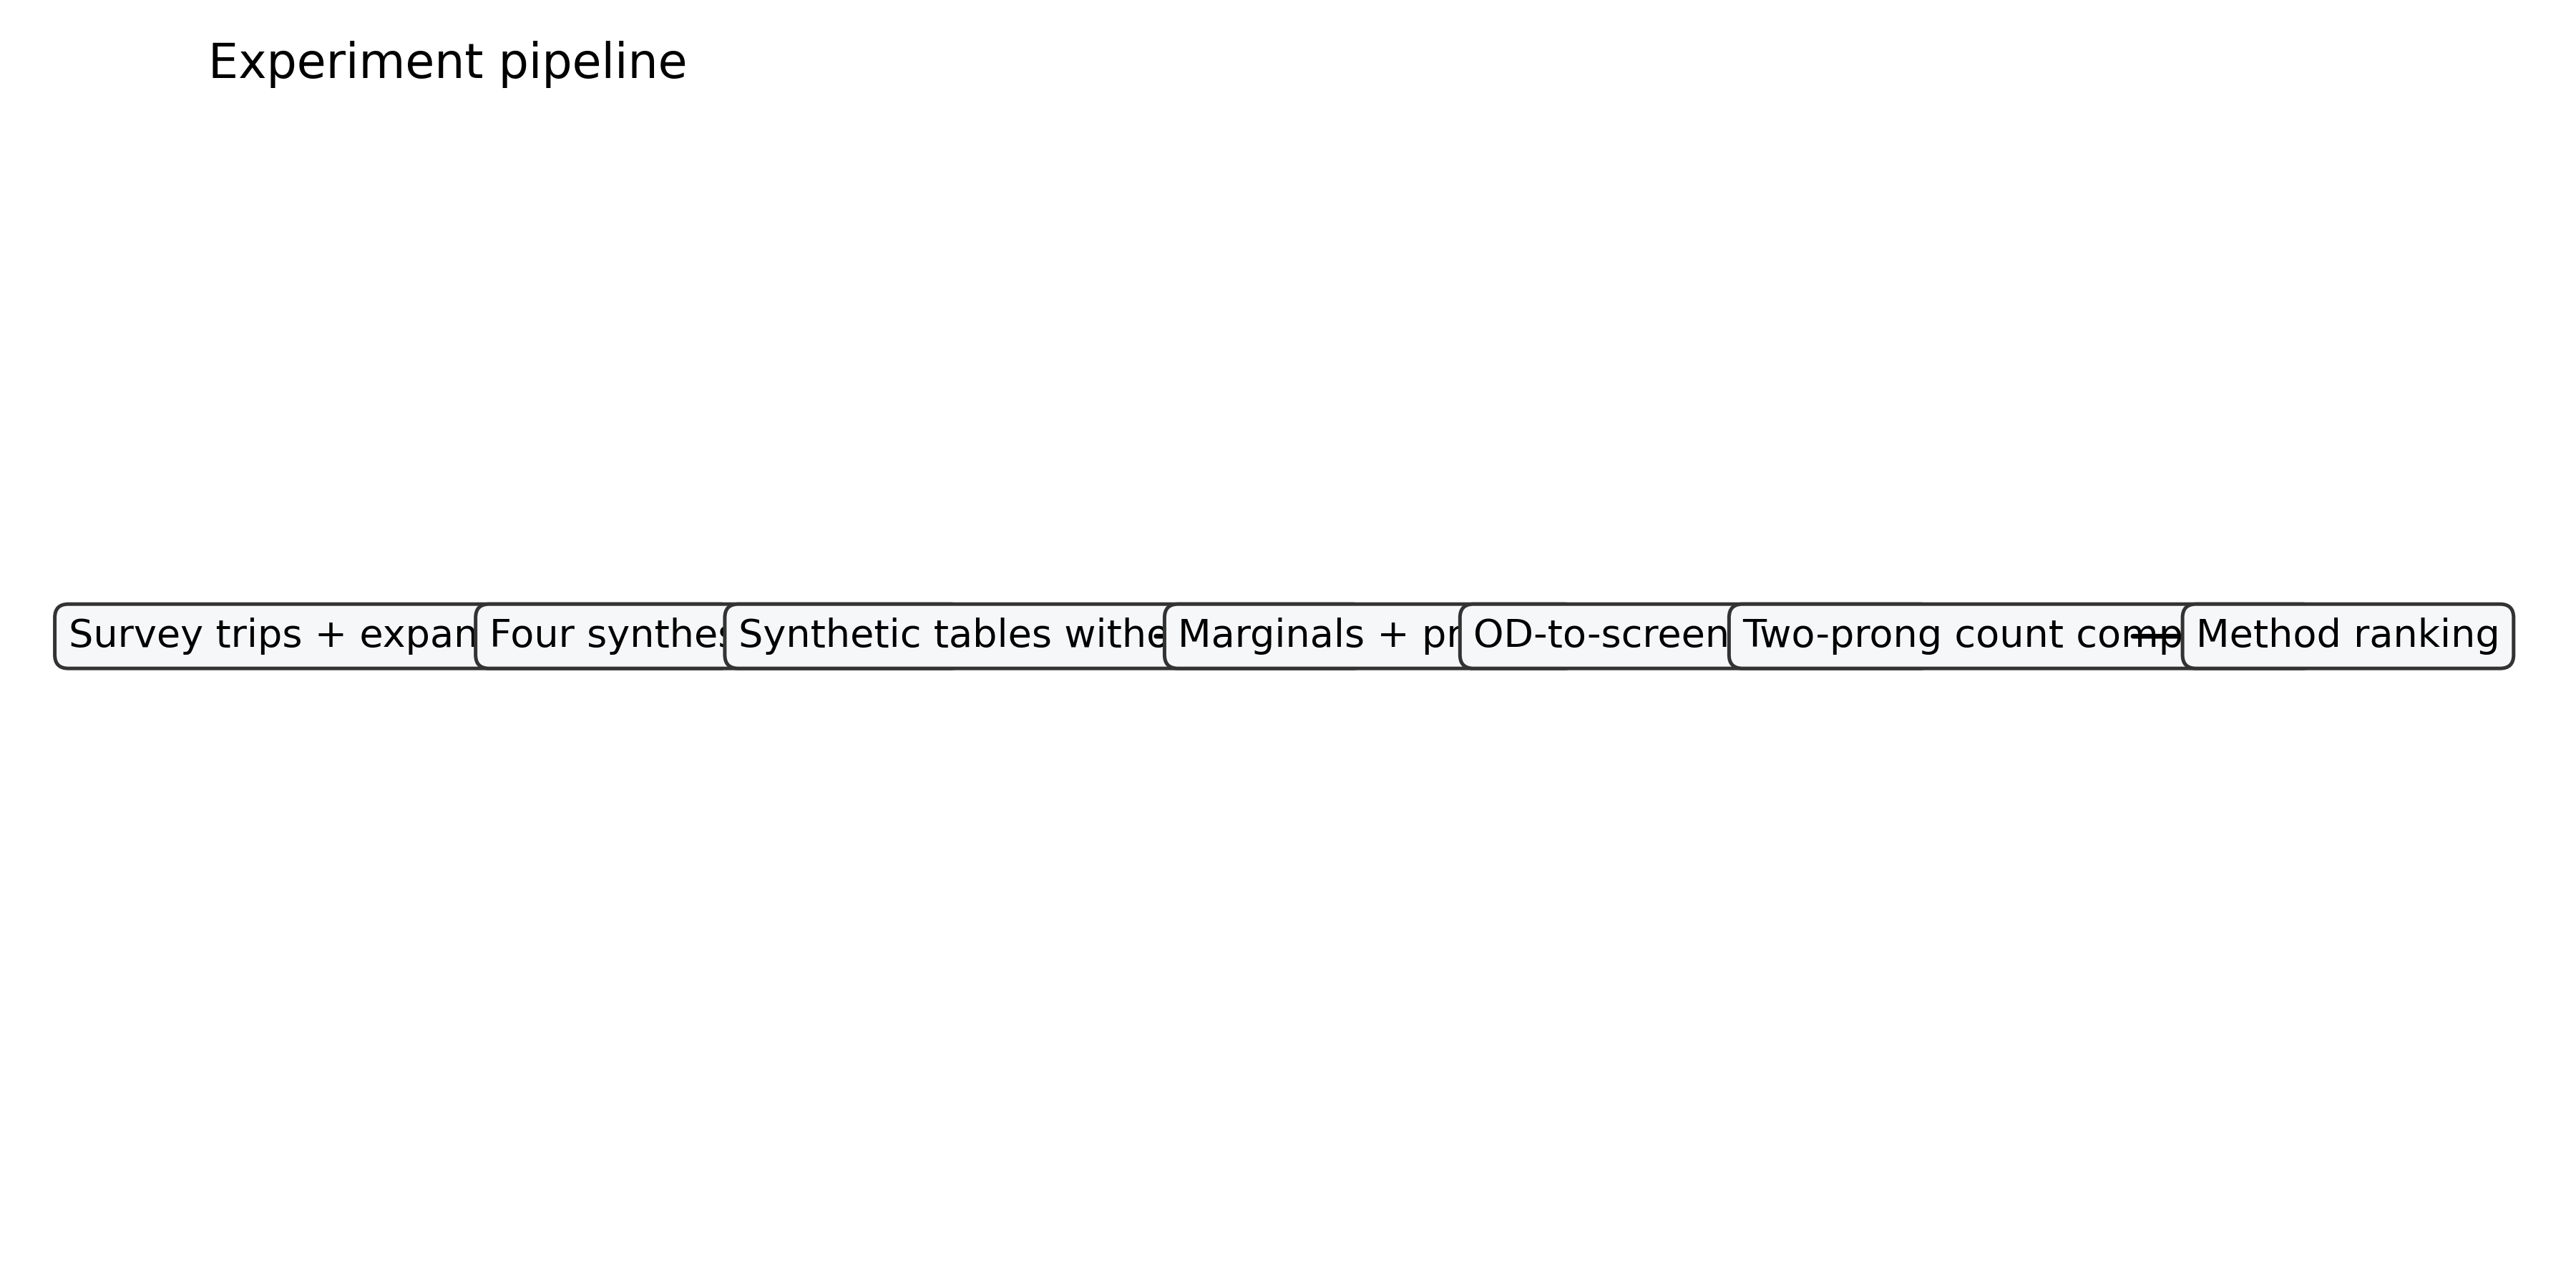
\includegraphics[width=.95\linewidth]{fig_experiment_pipeline.png}
\caption{\textbf{Implemented experiment pipeline.} The run proceeds from schema-bound survey input to four synthetic methods, internal distribution and privacy validation, and external two-prong screenline count validation.}
\label{fig:pipeline}
\end{figure}

\section{Contrastive Mixed-Tabular VAE}\label{sec:vae}
\subsection{Preprocessing and Architecture}
Let each trip record be represented as categorical fields $c$ and numeric fields $n$. A fitted preprocessor learns categorical vocabularies, numeric means, numeric standard deviations, numeric minima and maxima, and a stable feature order. Categorical values are mapped to integer codes; FIPS fields are cleaned before coding. Numeric fields are standardized as
\[
    \tilde n_{ij} = \frac{n_{ij}-\mu_j}{\sigma_j}.
\]
Missing numeric values are imputed by the training mean during transformation. During inverse transformation, numeric outputs are de-standardized, clipped to the training range by default, and rounded when the corresponding schema field is ordinal integer.

For each categorical column $j$ with $K_j$ levels, the encoder uses an embedding dimension
\[
    e_j =
    \begin{cases}
    1, & K_j \leq 1,\\
    \min\{32,\max[2,\mathrm{round}(4K_j^{1/4})]\}, & K_j > 1.
    \end{cases}
\]
In the fitted paper model, the embedding dimensions sum to \num{262}; concatenating the \num{18} numeric inputs gives an encoder input dimension of \num{280}. The encoder hidden sizes are \num{512}, \num{499}, \num{487}, and \num{475}, using linear layers, layer normalization, ReLU activations, and dropout of 0.02. The encoder outputs a \num{512}-dimensional latent mean vector $\mu$ and log-variance vector $\log\sigma^2$. The decoder mirrors the hidden stack in reverse and produces one numeric output head plus one softmax head for each categorical field. The model has approximately \num{8302216} trainable parameters.

\begin{figure}[H]
\centering
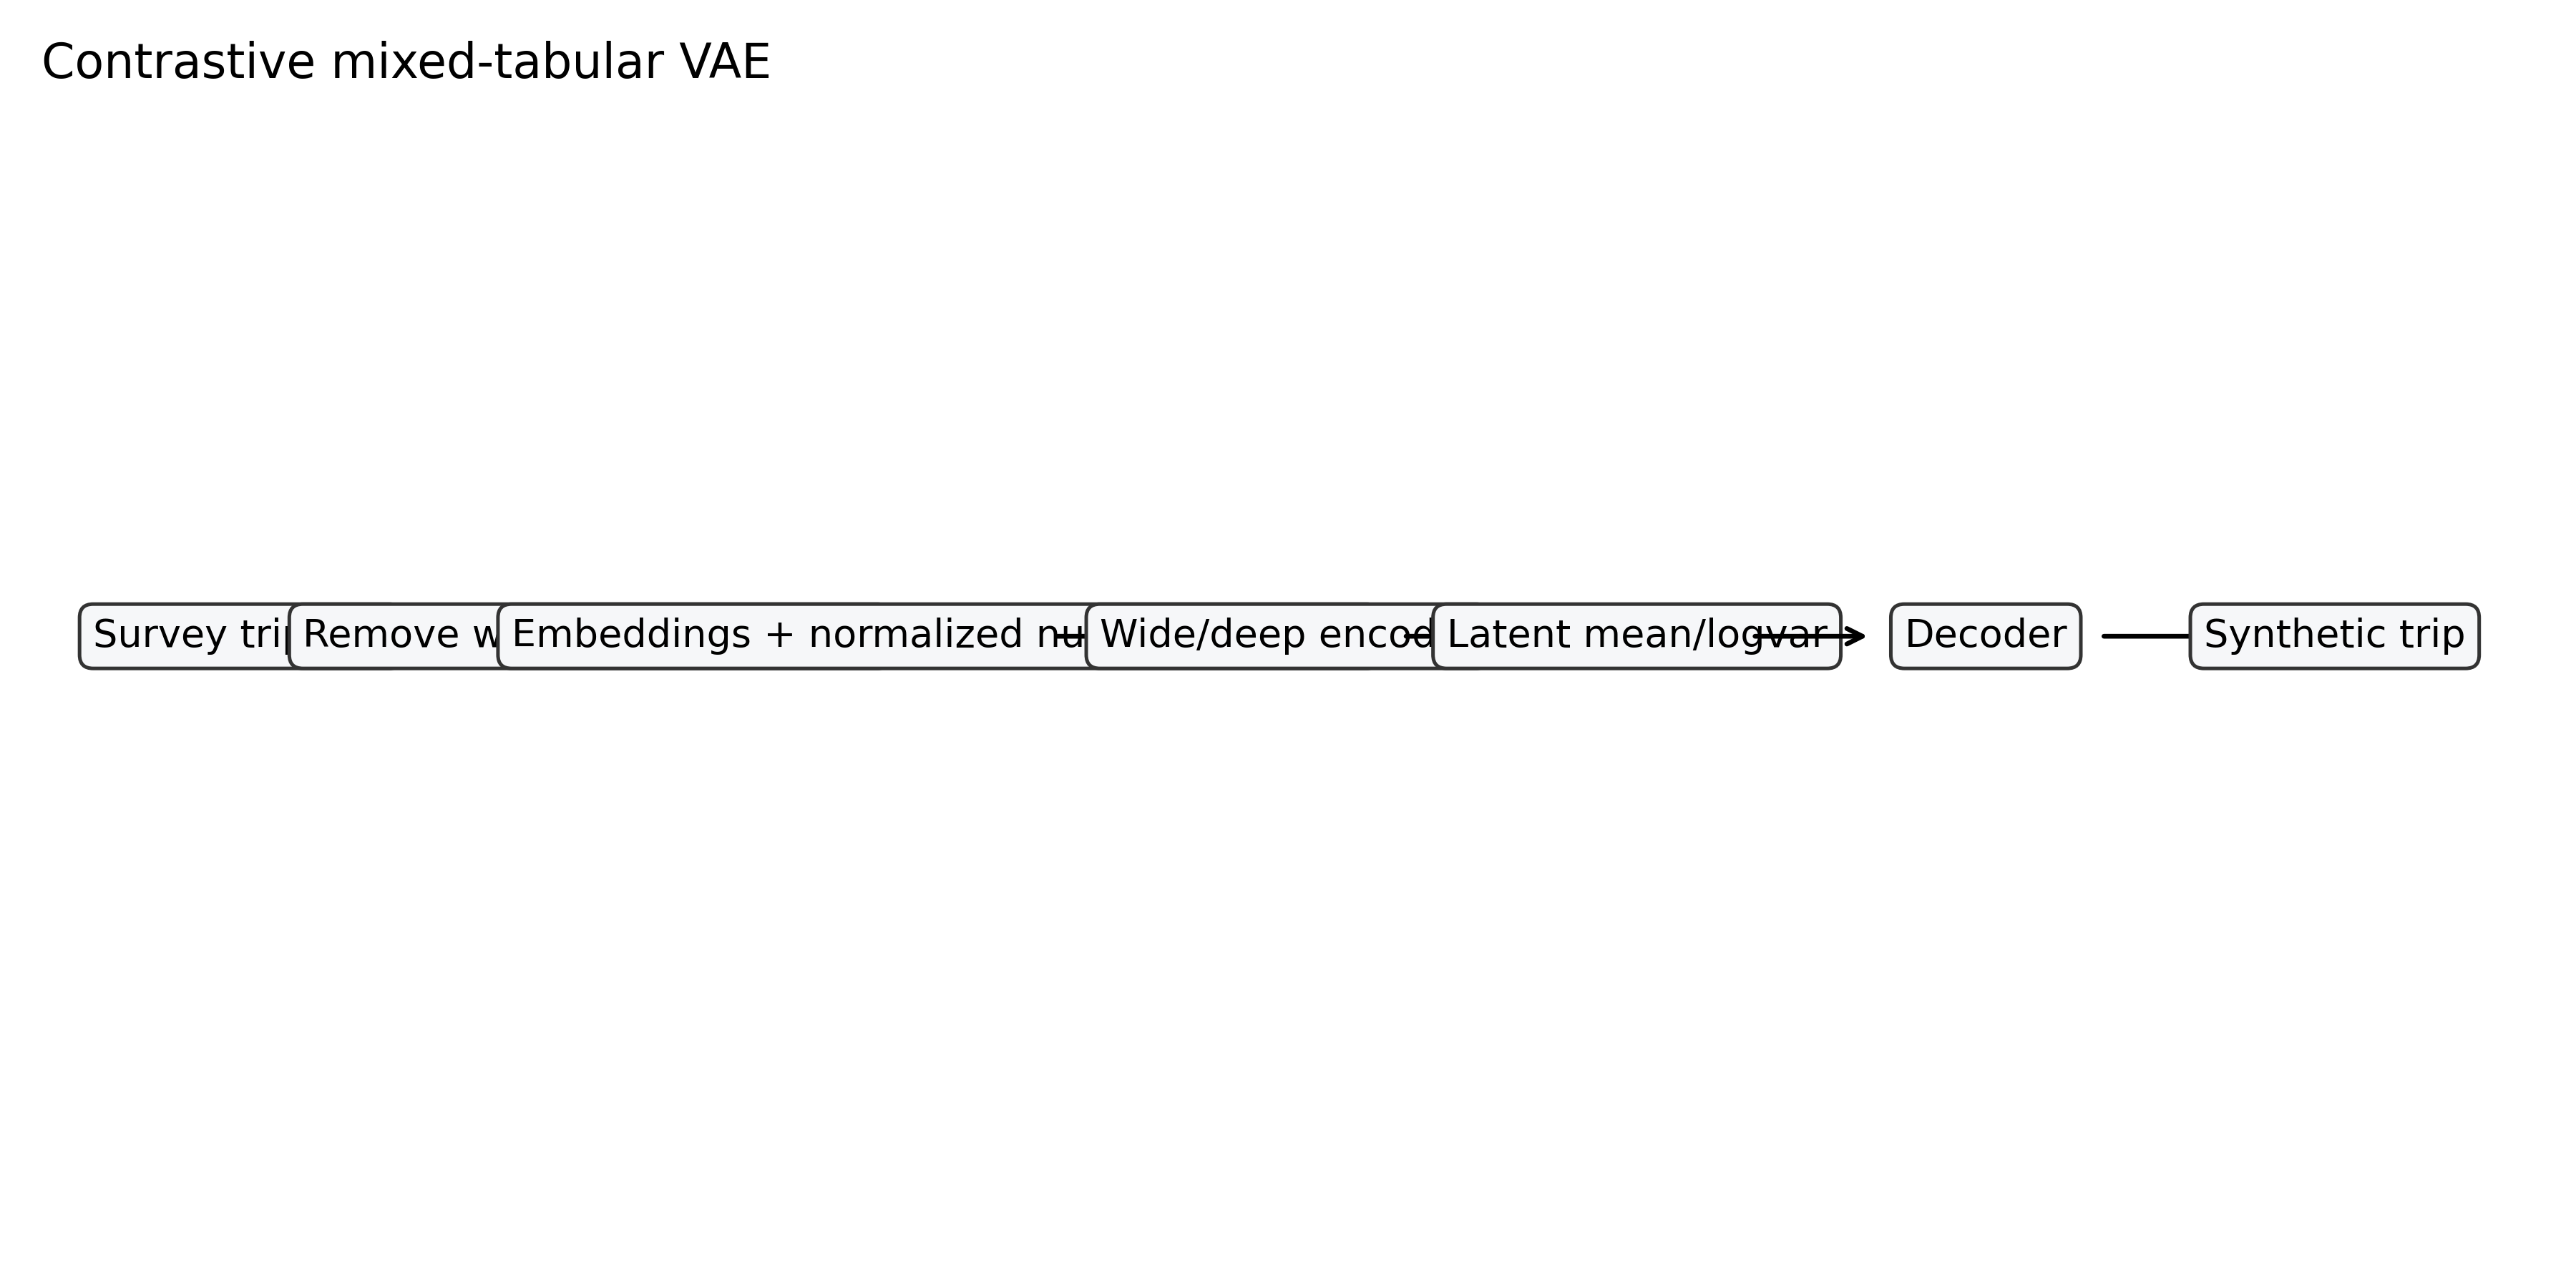
\includegraphics[width=.92\linewidth]{fig_architecture_contrastive_vae.png}
\caption{\textbf{Contrastive mixed-tabular VAE architecture.} Categorical fields are embedded, numeric fields are standardized, and the decoder uses column-specific categorical softmax heads plus a numeric reconstruction head.}
\label{fig:architecture}
\end{figure}

\begin{table}[H]
\centering
\caption{Final VAE configuration used for the paper run.}
\label{tab:vae-config}
\footnotesize
\begin{tabular}{ll}
\toprule
\textbf{Configuration item} & \textbf{Value} \\
\midrule
Latent dimension & \num{512} \\
Encoder/decoder depth & \num{4} hidden layers \\
Hidden sizes & \num{512}, \num{499}, \num{487}, \num{475} \\
Activation and normalization & ReLU with layer normalization \\
Dropout & 0.02 \\
Epoch limit & \num{1260} epochs \\
Batch size & \num{2048} \\
Optimizer and learning rate & AdamW, learning rate \num{0.0005} \\
KL coefficient $\beta$ & 0.03 \\
Contrastive coefficient $\lambda$ & 0.25 for contrastive VAE; 0.0 for noncontrastive VAE \\
Contrastive temperature $\tau$ & 0.10 \\
Positive view & Light corruption, protecting origin tract, destination tract, week, day-of-week, and departure time \\
Negative view & Marginal categorical corruption and within-batch numeric shuffling \\
Sampling temperature & 0.75 \\
Sampling chunk size & \num{25000} rows \\
Training weights & Survey weights capped at the 0.99 quantile and normalized to mean one \\
Random seed & \num{20260611} \\
\bottomrule
\end{tabular}
\end{table}

\subsection{Weighted Objective}
The model is trained on an 80/20 random train-validation split using seed \num{20260611}. Survey expansion weights are transformed before training. If $w_i$ is the original expansion weight, the implemented transform caps $w_i$ at the 99th percentile of positive weights and normalizes the resulting weights to mean one:
\[
    \tilde w_i =
    \frac{\min(w_i, q_{0.99})}{N^{-1}\sum_{k=1}^{N}\min(w_k, q_{0.99})}.
\]
The weighted row mean of any row loss $\ell_i$ is
\[
    \bar{\ell} = \frac{\sum_i \tilde w_i \ell_i}{\sum_i \tilde w_i}.
\]
This weighting lets high-expansion survey records influence the learned population distribution without making \texttt{weight} a generated field.

For each row, reconstruction loss is the sum of categorical cross-entropies and numeric mean-squared errors:
\[
    \ell^{rec}_i =
    \sum_{j \in \mathcal{C}}\mathrm{CE}\left(c_{ij}, \hat p_{ij}\right)
    +
    \sum_{k \in \mathcal{N}}\left(\tilde n_{ik}-\hat n_{ik}\right)^2.
\]
The KL term for a diagonal Gaussian posterior is
\[
    \ell^{KL}_i =
    -\frac{1}{2}\sum_{\ell=1}^{512}
    \left(1+\log\sigma_{i\ell}^2-\mu_{i\ell}^2-\sigma_{i\ell}^2\right).
\]
The noncontrastive VAE minimizes
\[
    \mathcal{L}_{VAE}
    =
    \overline{\ell^{rec}} + \beta\,\overline{\ell^{KL}},
    \qquad \beta=0.03.
\]

\subsection{Contrastive Regularization}
For the contrastive VAE, each batch also produces a positive and a negative view of the same records. The positive view lightly perturbs non-key categorical fields with probability 0.03 and jitters non-key numeric fields with Gaussian noise of scale 0.02. Origin tract, destination tract, survey week, survey day-of-week, and departure time are protected from positive corruption because they define the spatiotemporal trip identity. The negative view draws categorical codes from each marginal vocabulary and shuffles numeric values within the batch.

Let $z_i=\mu_i$ be the encoder mean for the original row, $z_i^+$ the encoder mean for its positive view, and $z_i^-$ the encoder mean for its negative view. With cosine similarity $s(\cdot,\cdot)$ and temperature $\tau=0.10$, the one-positive/one-negative InfoNCE term is
\[
    \ell^{con}_i =
    -\log
    \frac{\exp(s(z_i,z_i^+)/\tau)}
    {\exp(s(z_i,z_i^+)/\tau)+\exp(s(z_i,z_i^-)/\tau)}.
\]
The contrastive training objective is
\[
    \mathcal{L}_{CVAE}
    =
    \overline{\ell^{rec}}
    +
    \beta\,\overline{\ell^{KL}}
    +
    \lambda\,\overline{\ell^{con}},
    \qquad \lambda=0.25.
\]
The best contrastive checkpoint occurs at epoch \num{196}; the best noncontrastive checkpoint occurs at epoch \num{195}. Both methods were allowed to run to the configured \num{1260} epochs for comparable training histories, while sampling uses the saved best-validation checkpoint.

\begin{figure}[H]
\centering
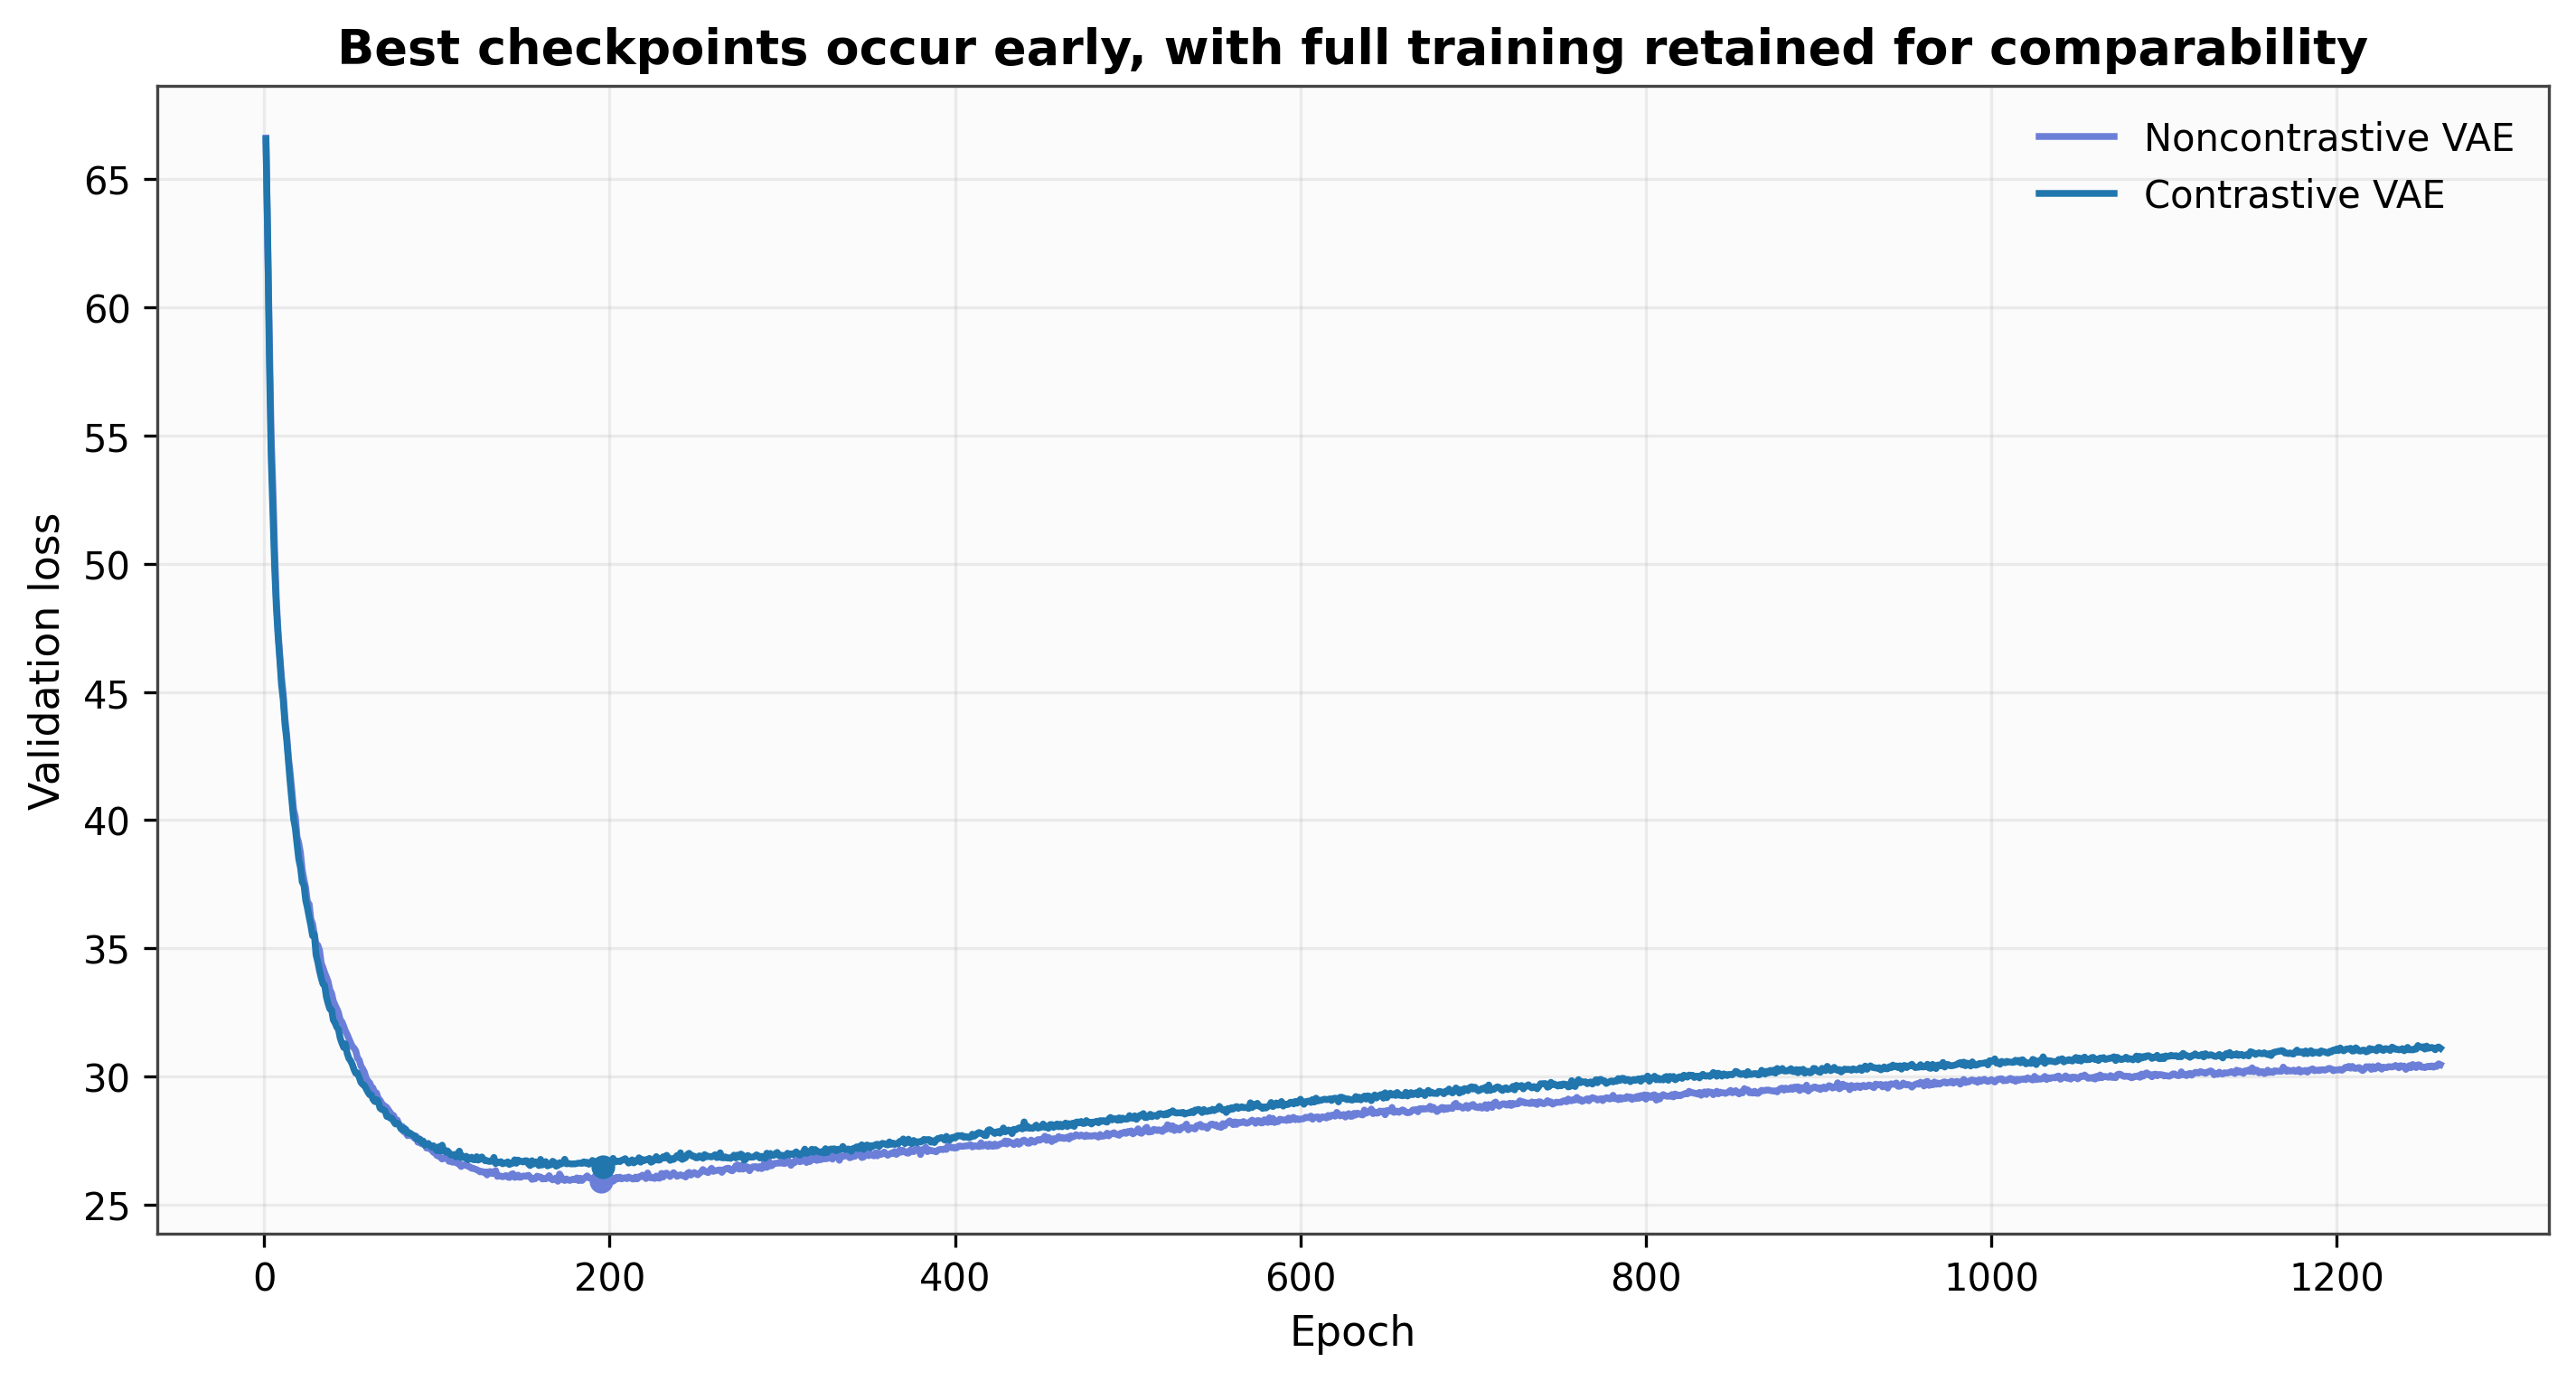
\includegraphics[width=.82\linewidth]{fig_vae_validation_loss_overlay.png}
\caption{\textbf{Validation-loss histories for the VAE ablation.} Both VAE variants reach their best validation checkpoint early, while the configured run retains the full epoch budget.}
\label{fig:training-history}
\end{figure}

\subsection{Sampling}
Synthetic rows are generated by drawing $z\sim\mathcal{N}(0,I)$, decoding through the VAE, sampling categorical codes from temperature-scaled softmax distributions, inverse-transforming numeric values, clipping numeric values to training ranges, and applying the synthetic data contract. The output contains all modeled features plus \texttt{synthetic\_method} and \texttt{synthetic\_run\_id}. It never contains \texttt{weight}. The one-million-row cap is a file-size and runtime decision; traffic-count validation uses each method's stored expansion factor to represent the full weighted target.

\section{Validation Design}\label{sec:validation}
\subsection{Internal Distribution Validation}
Internal validation compares the real survey table with each synthetic table using the fitted reference preprocessor's feature list. Survey-side estimates are weighted by \texttt{weight}; synthetic-side estimates are unweighted because generated rows represent the synthetic analysis population.

For categorical fields, the pipeline computes weighted survey proportions, synthetic proportions, total variation distance, Jensen-Shannon distance, and the largest category errors. For numeric fields, it computes weighted survey summaries, synthetic summaries, mean error, standard-deviation error, one-dimensional Wasserstein distance, and Kolmogorov-Smirnov statistic. The method-level marginal similarity score is
\[
    S_{marg} = 1-\mathrm{mean}\left(\TVD_{\mathrm{cat}}, KS_{\mathrm{num}}\right).
\]

Cross-marginal validation tests selected two-way relationships that matter for trip synthesis: origin activity by destination activity, travel mode by departure-time bin, origin county by destination county, day-of-week by departure-time bin, household income by vehicle occupancy, origin activity by mode, destination activity by mode, distance bin by reported-travel-time bin, and vehicle model year by vehicle. The method-level cross-marginal similarity score is $1-\mathrm{mean}(\TVD_{\mathrm{cross}})$.

\subsection{Copying and Validity Diagnostics}
Privacy diagnostics compute exact-row copy rate against the real feature table, duplicate rate within the synthetic table, invalid categorical value rate, novel origin-destination pair share, and a simple non-copying score
\[
    S_{privacy}=1-\mathrm{copy\_rate}-\mathrm{invalid\_category\_rate}.
\]
This is not differential privacy. It is a computationally scalable diagnostic intended to prevent copied records from being mistaken for generative fidelity. Nearest-neighbor privacy scans are disabled in the paper run because an all-pairs synthetic-by-real scan is not practical at one million synthetic rows.

\subsection{Two-Prong Screenline Count Validation}
The external validation uses 2019 Census TIGER/Line tracts for Maryland, DC, and Virginia \cite{uscensus_tiger_2019}, filtered to tract GEOIDs appearing in survey origin, destination, home, or work fields. MDOT SHA AADT station points provide dense annual-average count locations and annual-average weekday traffic fields \cite{mdot_aadt_2019}. FHWA TMAS station files provide sparse but temporally detailed station-hour counts \cite{fhwa_tmas_data}. In the local processed files, FHWA TMAS contributes \num{64} continuous-count stations, \num{37800} station-day rows, and \num{907200} station-hour rows over \num{665} dates.

The screenline construction is geometric. Adjacent tract pairs are found from shared tract boundaries. A tract boundary becomes a candidate screenline if it is within the observed-station buffer scope. A station is assigned to a screenline only when its distance to the shared boundary is less than half its distance to the nearer adjacent tract centroid. The resulting paper run contains \num{2232} filtered tracts, \num{5927} adjacent tract pairs, \num{3257} candidate screenlines, \num{3107} screenlines with stations, and \num{6725} station-to-screenline assignments. Figure~\ref{fig:screenline-concept} illustrates the tract-boundary validation concept.

\begin{figure}[H]
\centering
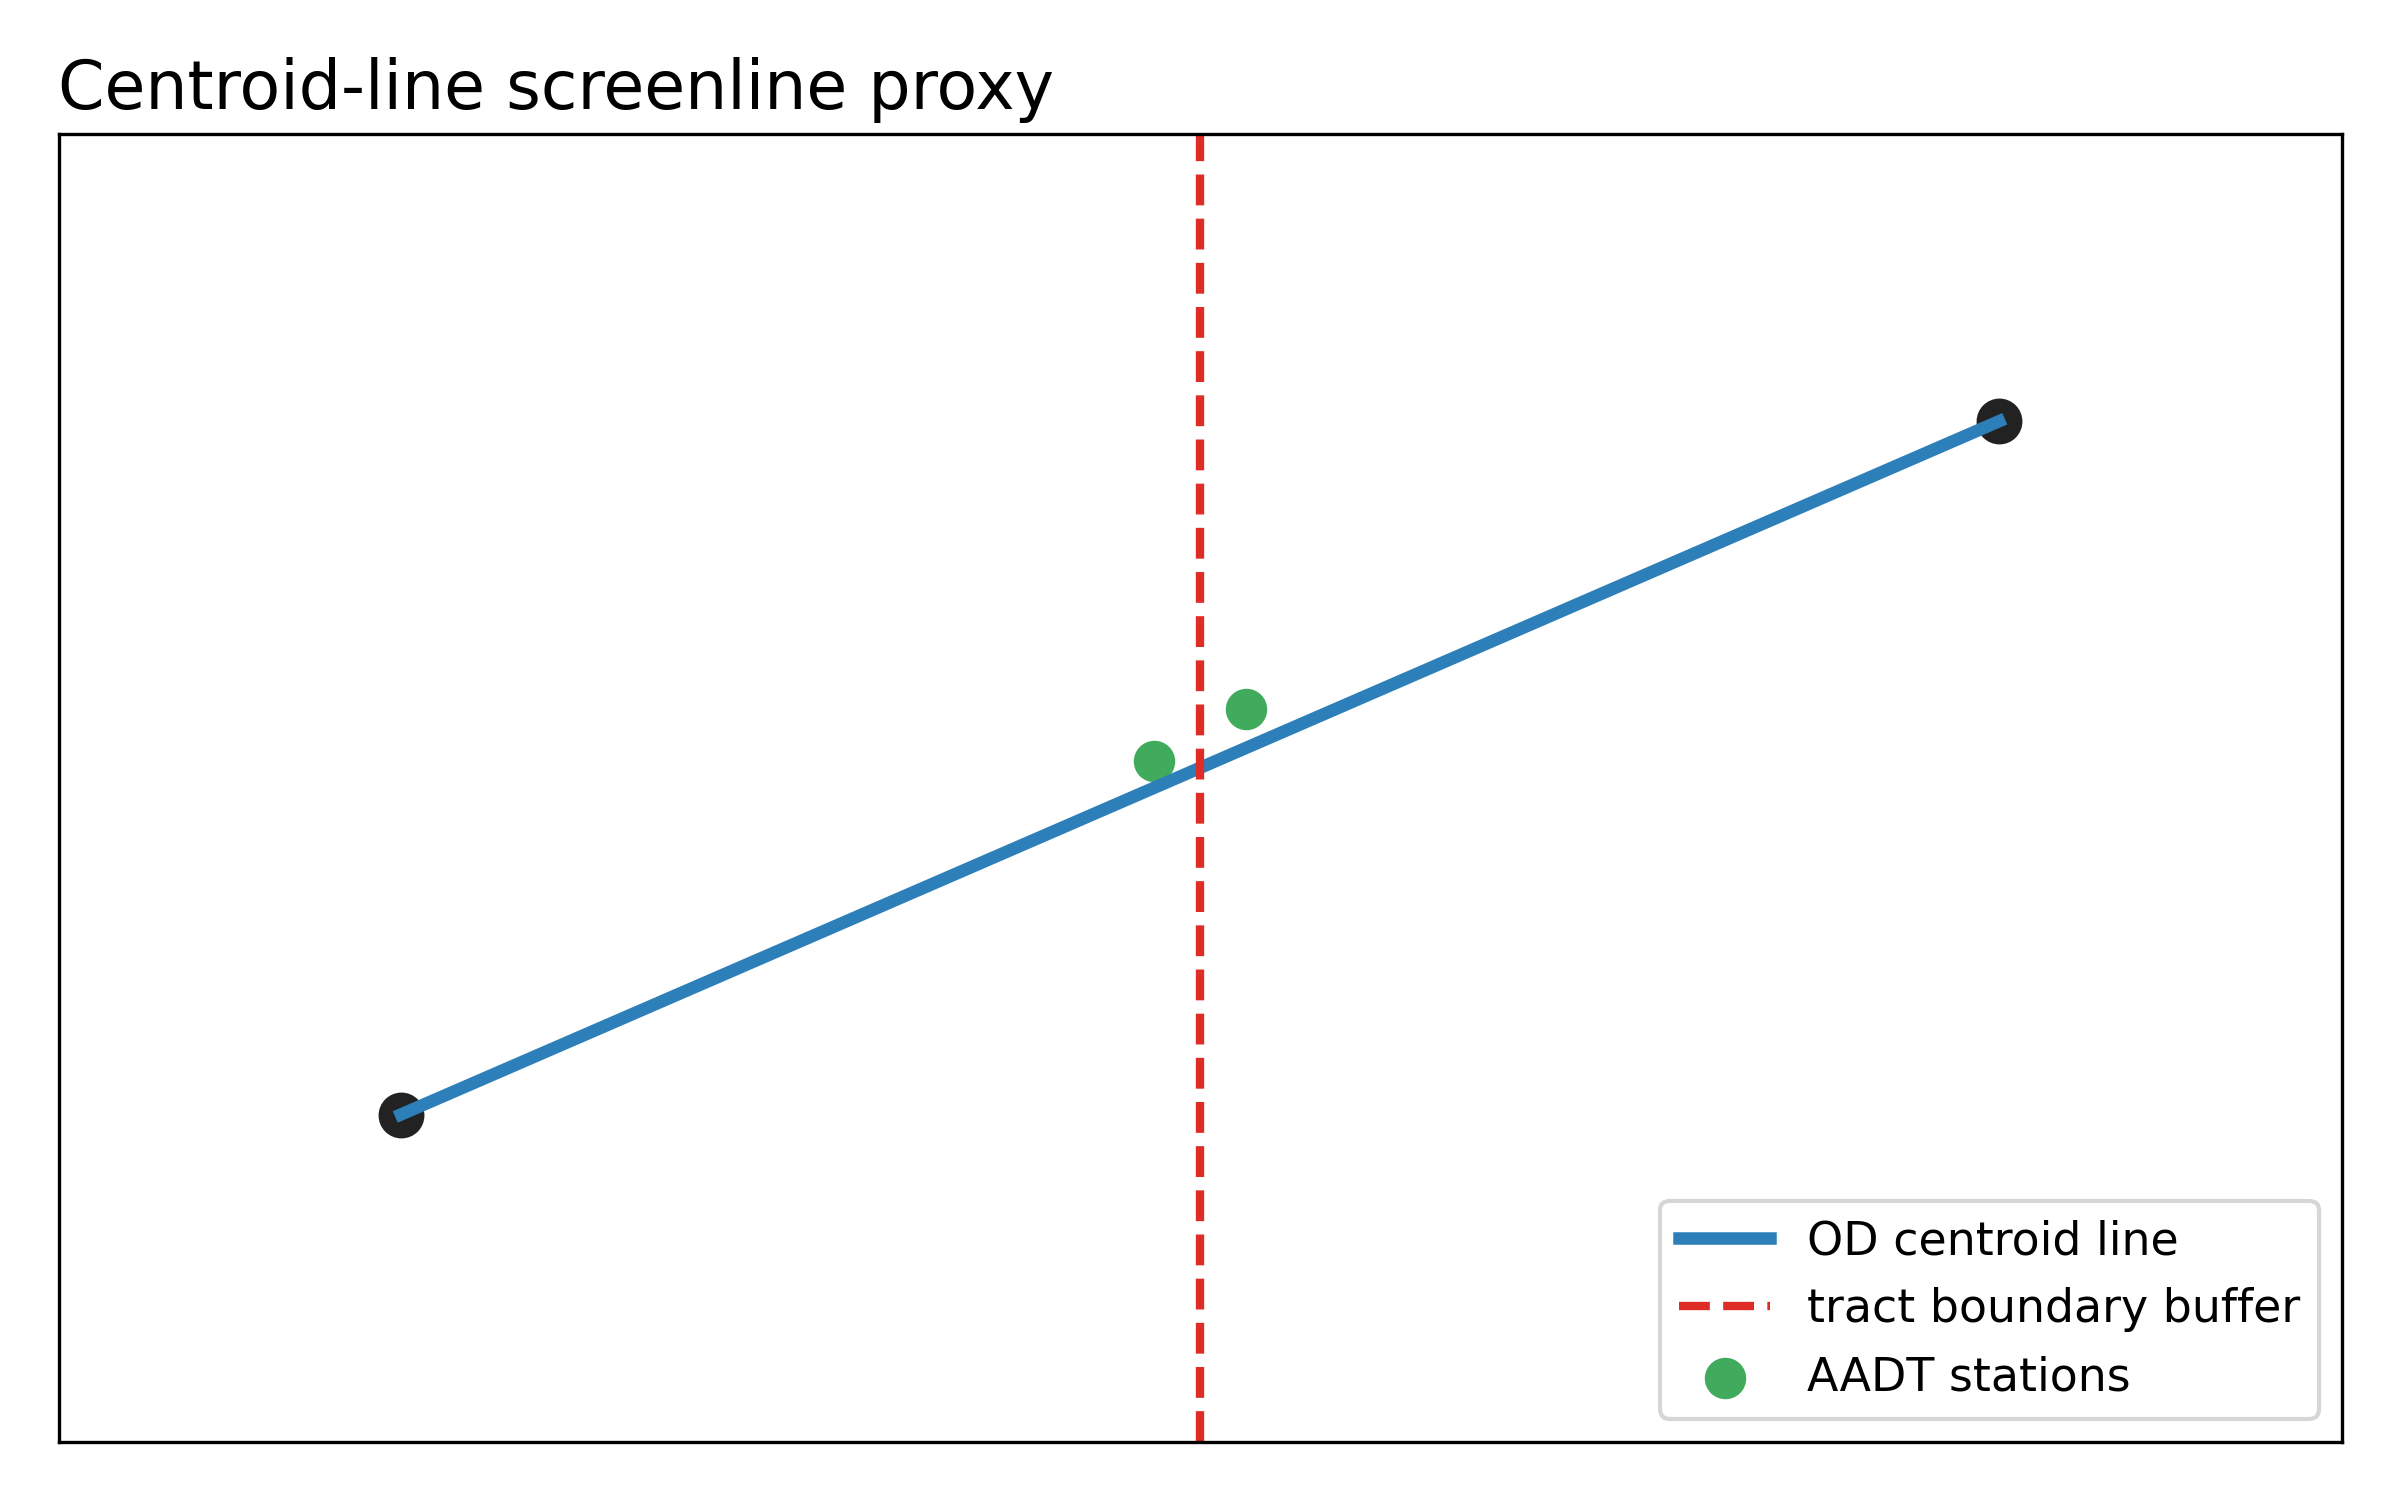
\includegraphics[width=.82\linewidth]{fig_screenline_concept_map.png}
\caption{\textbf{Screenline validation concept.} The method maps tract-boundary screenlines to nearby MDOT traffic-count stations and counts synthetic virtual crossings along tract-representative-point OD paths.}
\label{fig:screenline-concept}
\end{figure}

For each origin-destination tract pair, the path proxy is a straight line between tract representative points. The ordered tract crossings along this line are converted into screenline crossings. This is intentionally not a full network assignment. It is a transparent geographic proxy for testing whether synthetic OD structure produces plausible aggregate boundary crossings.

The annual tier compares synthetic long-term average screenline crossings with dense MDOT annual-average counts. Synthetic trip dates are reconstructed from \texttt{tdate\_week} and \texttt{tdate\_dow}, where weeks are offsets from January 1, 2017 and day-of-week follows ISO Monday=1, Sunday=7. Date-stratified synthetic counts are expanded by reconstructed date count because the survey weights are interpreted as average-day expansion weights.

The hourly tier compares synthetic hourly crossings with FHWA TMAS station-hour counts scaled to screenline totals. If station $s$ has annual count $A_s$ and screenline $L$ has total annual count $A_L$, the station's annual share is
\[
    p_{sL}=\frac{A_s}{A_L}.
\]
For each screenline-hour cell, observed screenline traffic is estimated as
\[
    O_{Lth}=\frac{\sum_{s\in L} H_{sth}}{\sum_{s\in L}p_{sL}},
\]
where $H_{sth}$ is the FHWA TMAS hourly station count. Synthetic crossing time is estimated by placing each screenline crossing along the trip's reported travel time:
\[
    t^{cross}_{i\ell}=t^{dep}_i+r_i\frac{k_\ell+1}{K_i+1},
\]
where $r_i$ is reported travel time, $k_\ell$ is the zero-indexed crossing position, and $K_i$ is the number of crossings for trip $i$.

Both tiers report raw and log correlations, RMSE, MAE, guarded MAPE, SMAPE, median APE, mean bias, $R^2$, GEH statistics, and calibration slope/intercept. The traffic-count framing follows the broader FHWA traffic monitoring context, in which continuous and short-duration count programs are used to produce and quality-control annual and temporal volume estimates \cite{fhwa_traffic_monitoring_guide}. The GEH statistic is computed as
\[
    GEH = \sqrt{\frac{2(S-O)^2}{S+O}},
\]
where $S$ and $O$ are synthetic and observed counts.

\section{Results}\label{sec:results}
\subsection{Internal Fidelity, Copying, and Novelty}
Table~\ref{tab:internal-results} and Figure~\ref{fig:internal-scores} summarize internal validation. Weighted bootstrap has the strongest one-way and two-way internal fit because it resamples observed records, but its exact-row copy rate is 1.0 and its duplicate rate is 0.8918. This is the essential baseline: it shows the upper bound for distributional overlap obtainable by copying and the privacy/diversity cost of that strategy.

The Bayesian network closely matches one-way marginals but loses more cross-marginal structure, as expected from a tree-structured approximation. Both VAE variants avoid exact copying and invalid categories. The contrastive VAE improves mean numeric KS from 0.1261 to 0.1103 and mean cross-marginal TV from 0.2556 to 0.2265 relative to the noncontrastive VAE. The cost is a small increase in mean categorical TV from 0.0621 to 0.0652. In other words, the contrastive regularizer improves joint behavioral structure and numeric fidelity while slightly weakening average categorical marginal fit.

\begin{table}[H]
\centering
\caption{Internal validation summary. Lower is better for TV, KS, copy rate, and duplicate rate; higher is better for similarity and novel OD support when invalid-category rate remains zero.}
\label{tab:internal-results}
\footnotesize
\begin{tabular}{lrrrrrrr}
\toprule
\textbf{Method} & \textbf{Cat. TV} & \textbf{Num. KS} & \textbf{Marg. sim.} & \textbf{Cross TV} & \textbf{Cross sim.} & \textbf{Copy} & \textbf{Novel OD} \\
\midrule
Weighted bootstrap & 0.0033 & 0.0439 & 0.9801 & 0.0050 & 0.9950 & 1.0000 & 0.0000 \\
Bayesian network & 0.0034 & 0.0437 & 0.9801 & 0.0901 & 0.9099 & 0.0000 & 0.3330 \\
Noncontrastive VAE & 0.0621 & 0.1261 & 0.9117 & 0.2556 & 0.7444 & 0.0000 & 0.6856 \\
Contrastive VAE & 0.0652 & 0.1103 & 0.9163 & 0.2265 & 0.7735 & 0.0000 & 0.6852 \\
\bottomrule
\end{tabular}
\end{table}

\begin{figure}[H]
\centering
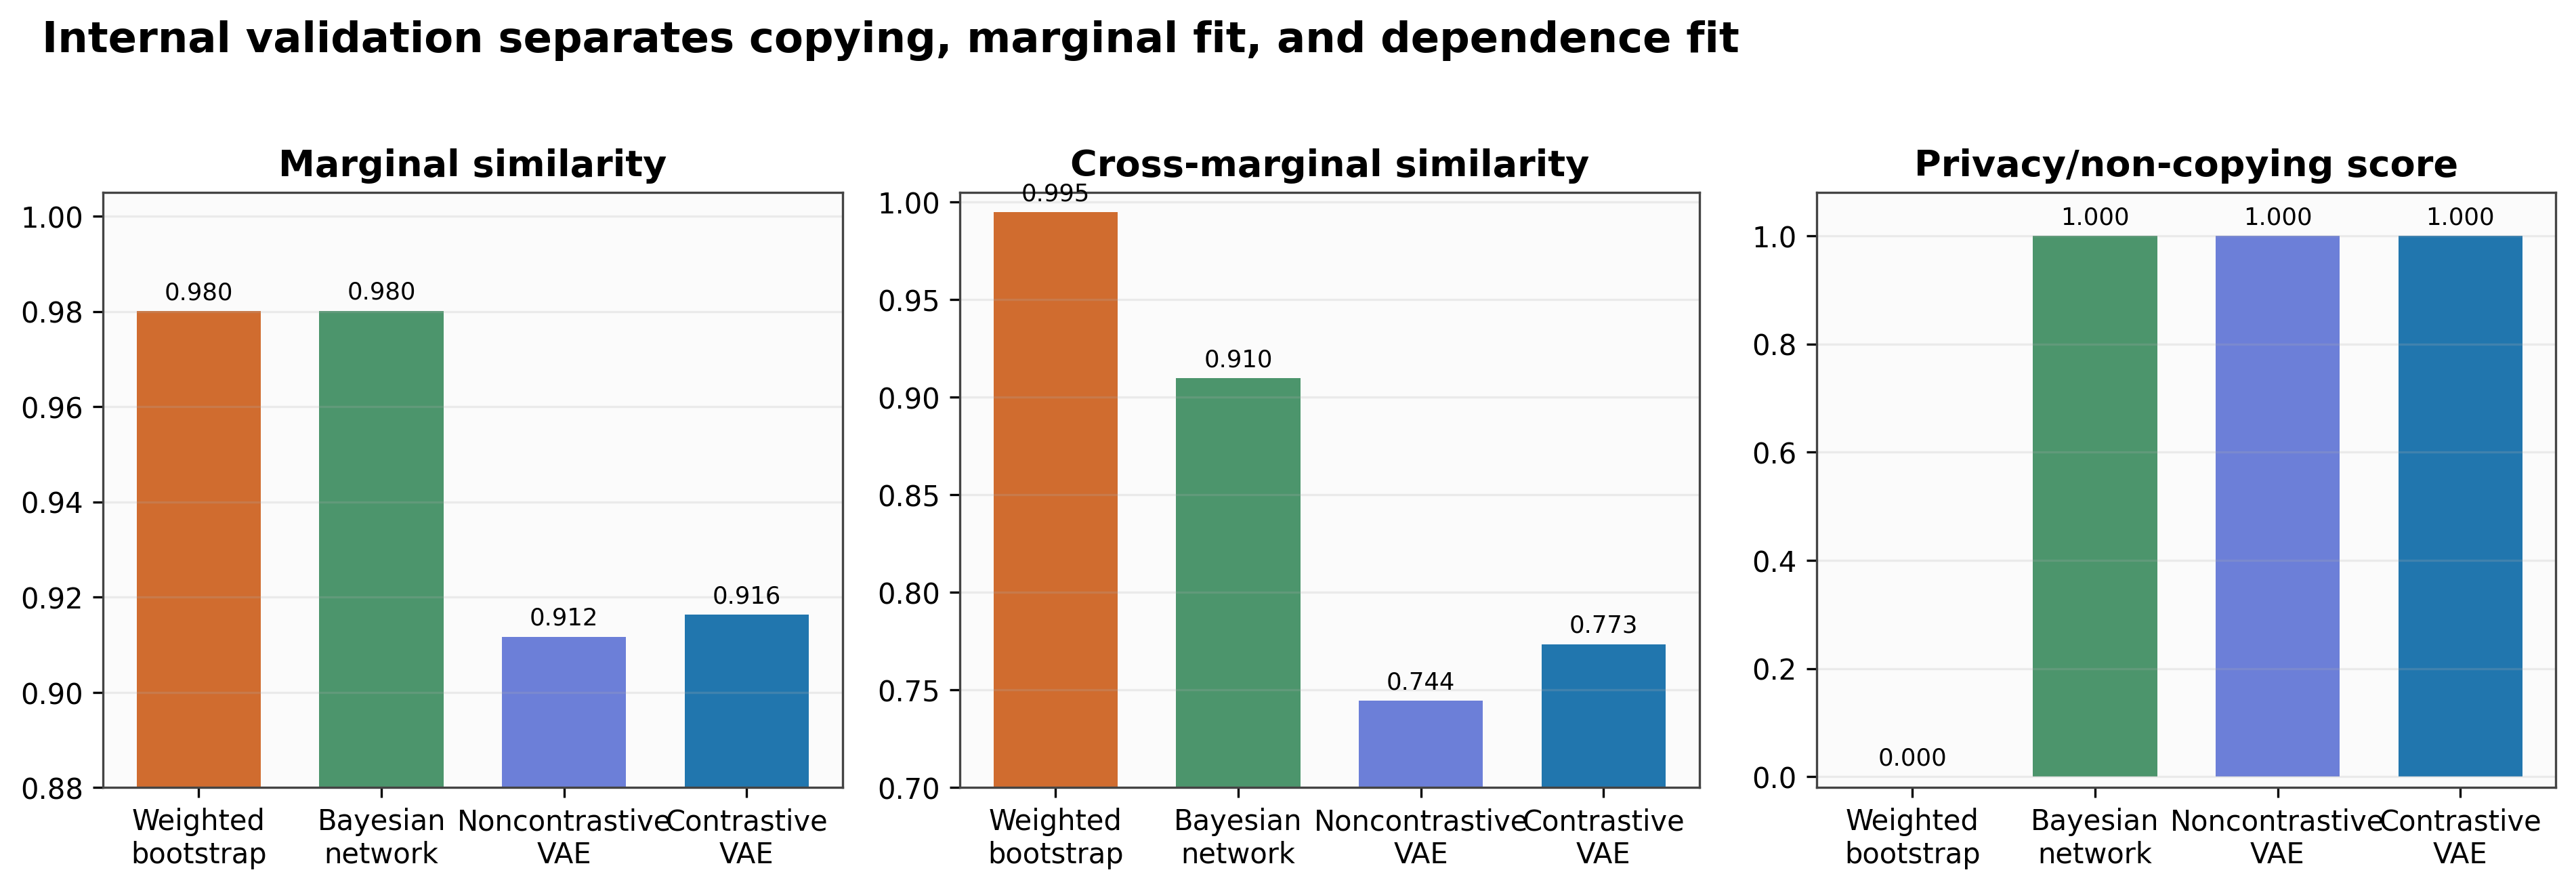
\includegraphics[width=.95\linewidth]{fig_internal_validation_scores.png}
\caption{\textbf{Internal validation scores.} Bootstrap dominates marginal and cross-marginal scores by copying; the learned generators avoid exact row copying, with the contrastive VAE improving dependence fit over the noncontrastive VAE.}
\label{fig:internal-scores}
\end{figure}

\begin{figure}[H]
\centering
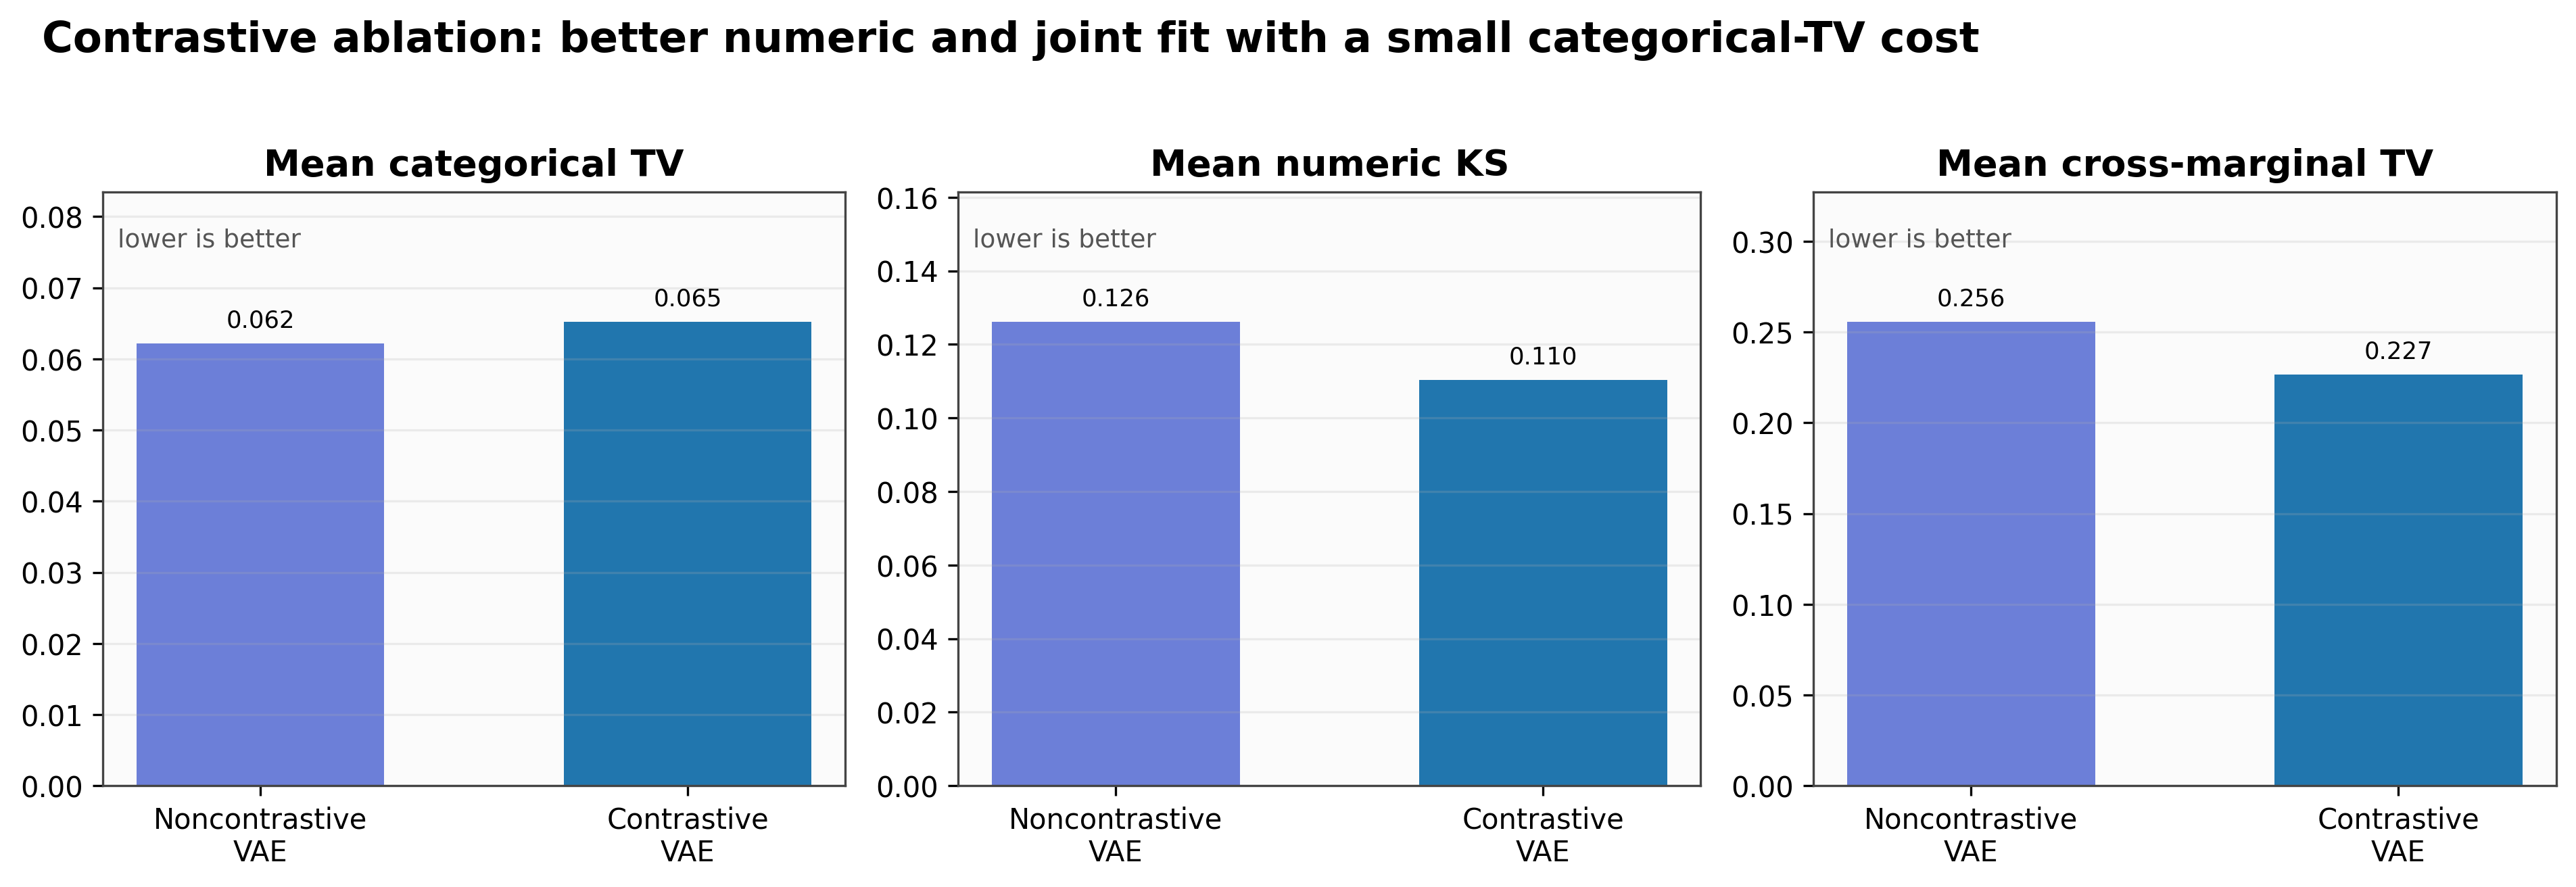
\includegraphics[width=.95\linewidth]{fig_contrastive_ablation_errors.png}
\caption{\textbf{Contrastive ablation.} Relative to the noncontrastive VAE, the contrastive VAE reduces numeric KS and cross-marginal TV while slightly increasing categorical TV.}
\label{fig:ablation}
\end{figure}

\subsection{Origin-Destination Support}
The survey input contains \num{58925} unique directed origin-destination tract pairs. The weighted bootstrap sample contains \num{58009}, essentially reproducing the observed support. The Bayesian network generates \num{180910} unique directed pairs. The noncontrastive and contrastive VAEs generate \num{398039} and \num{395542}, respectively, unique directed pairs in their one-million-row samples. This is the clearest sign that the VAE is not simply memorizing the survey's observed OD table. The key question then becomes whether this broader support remains distributionally and externally plausible.

\begin{figure}[H]
\centering
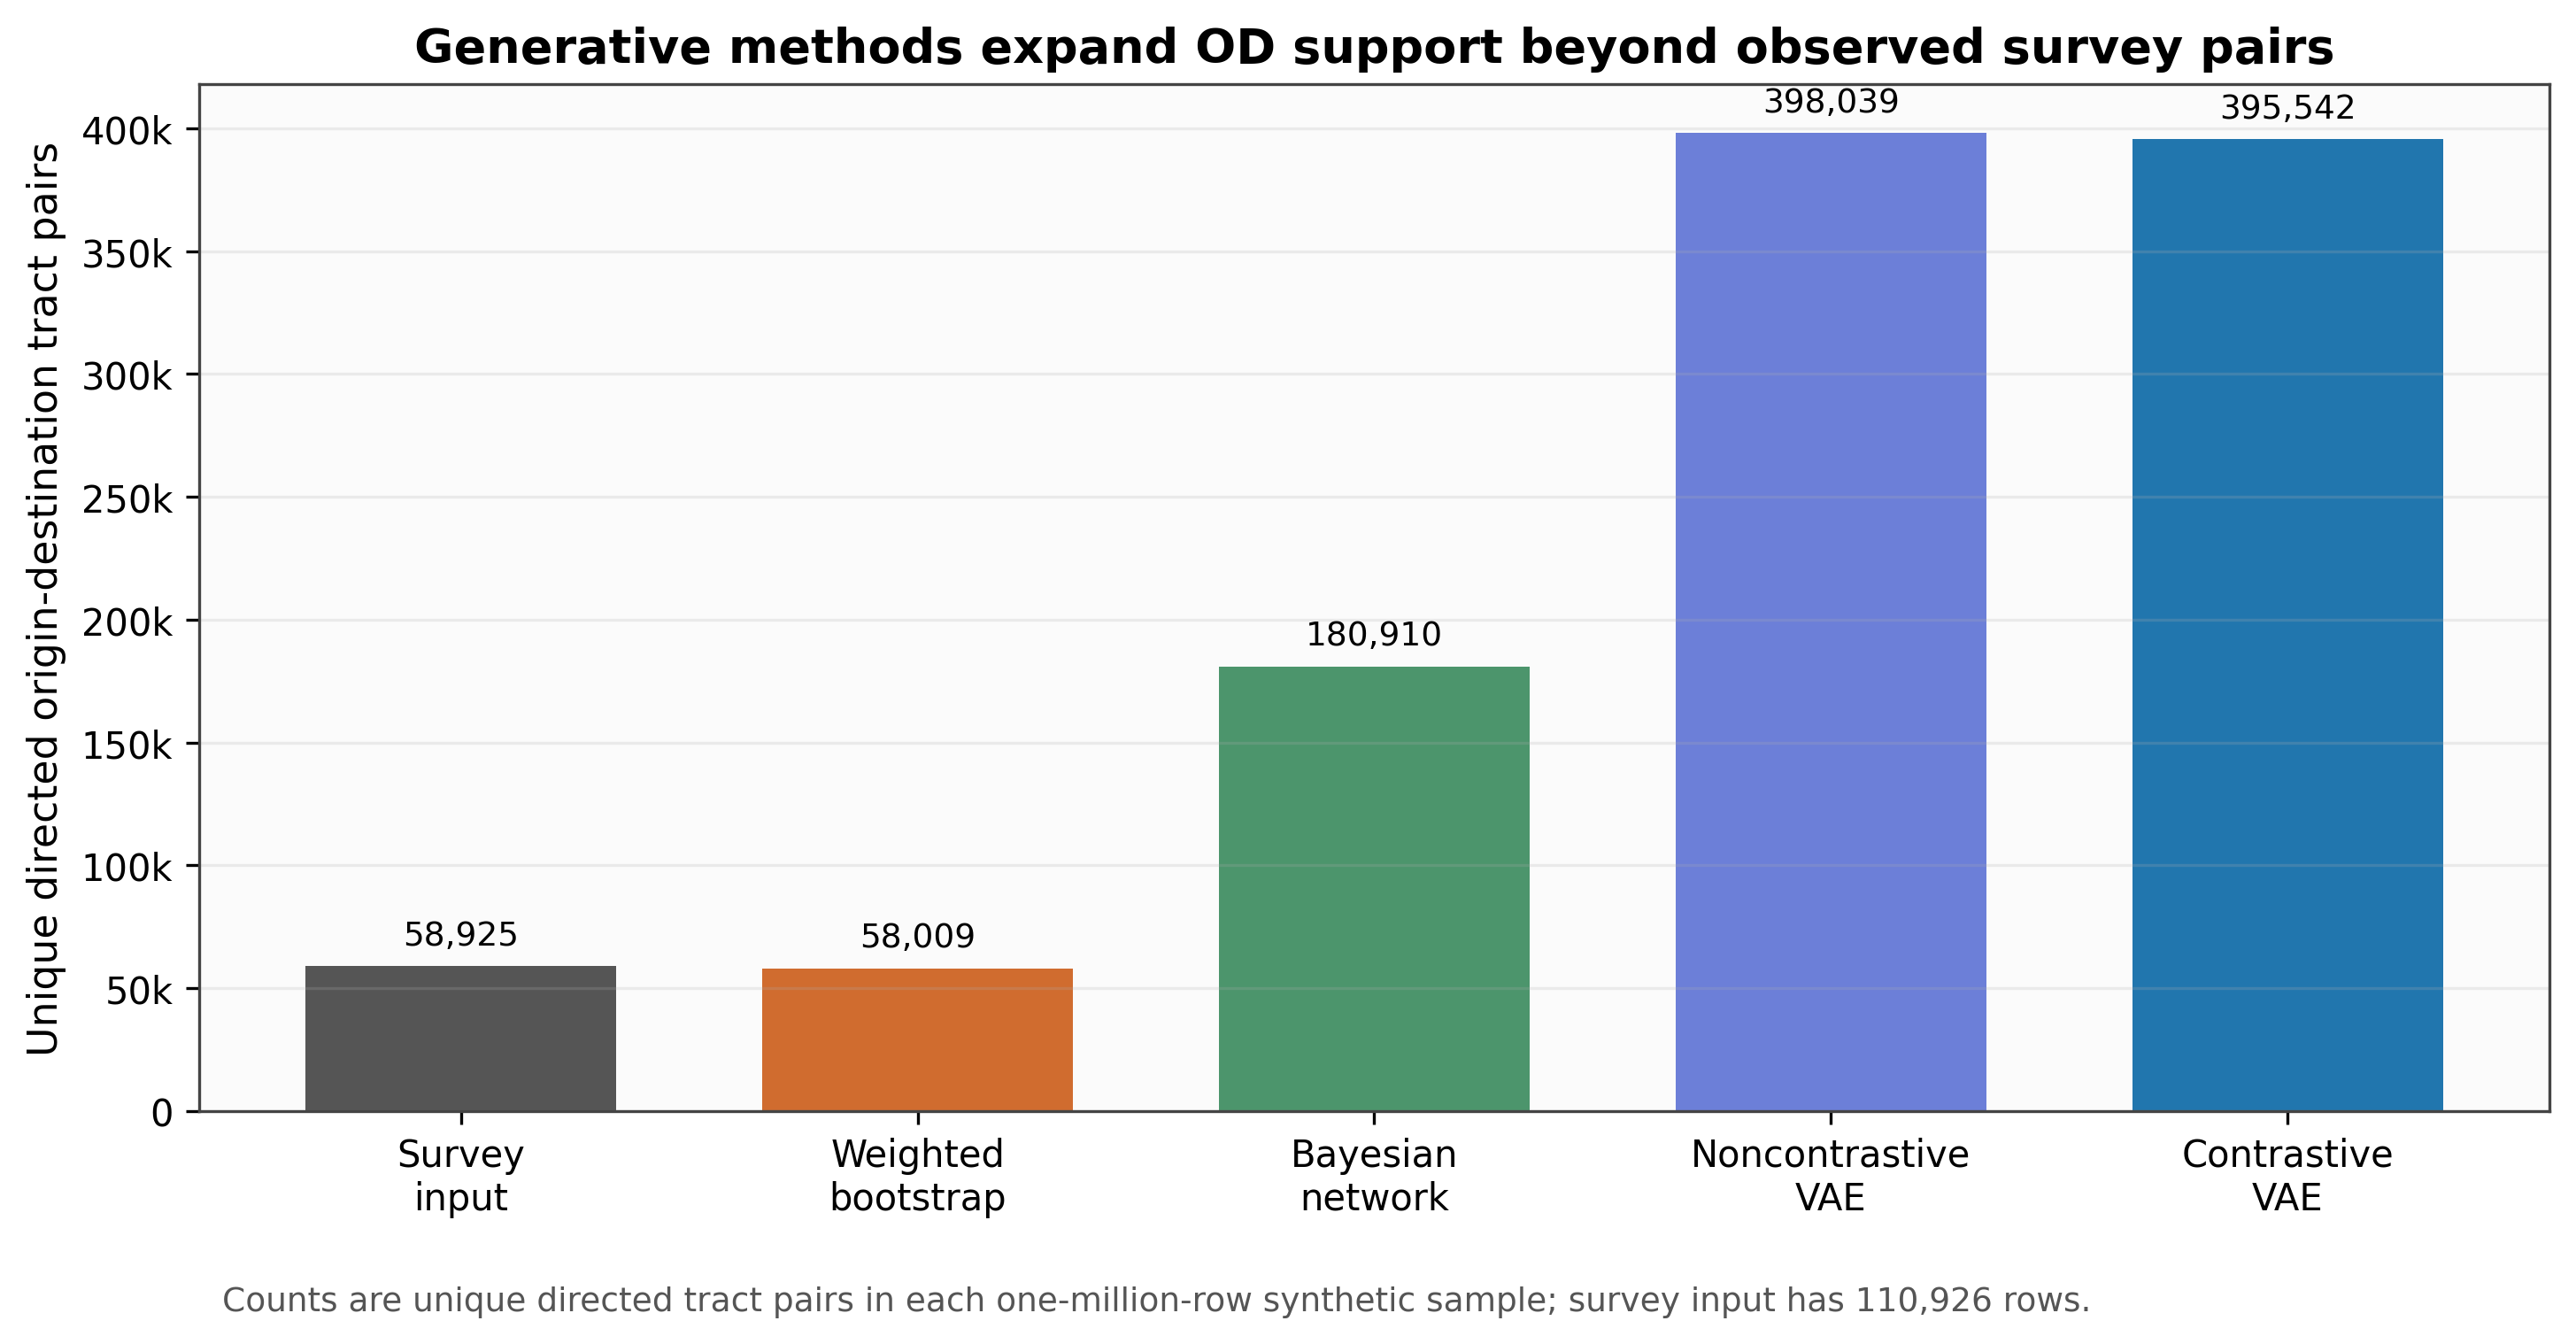
\includegraphics[width=.82\linewidth]{fig_od_support_unique_pairs.png}
\caption{\textbf{Unique directed origin-destination tract support.} Learned generators greatly expand OD support relative to the observed survey table and the bootstrap baseline.}
\label{fig:od-support}
\end{figure}

\begin{figure}[H]
\centering
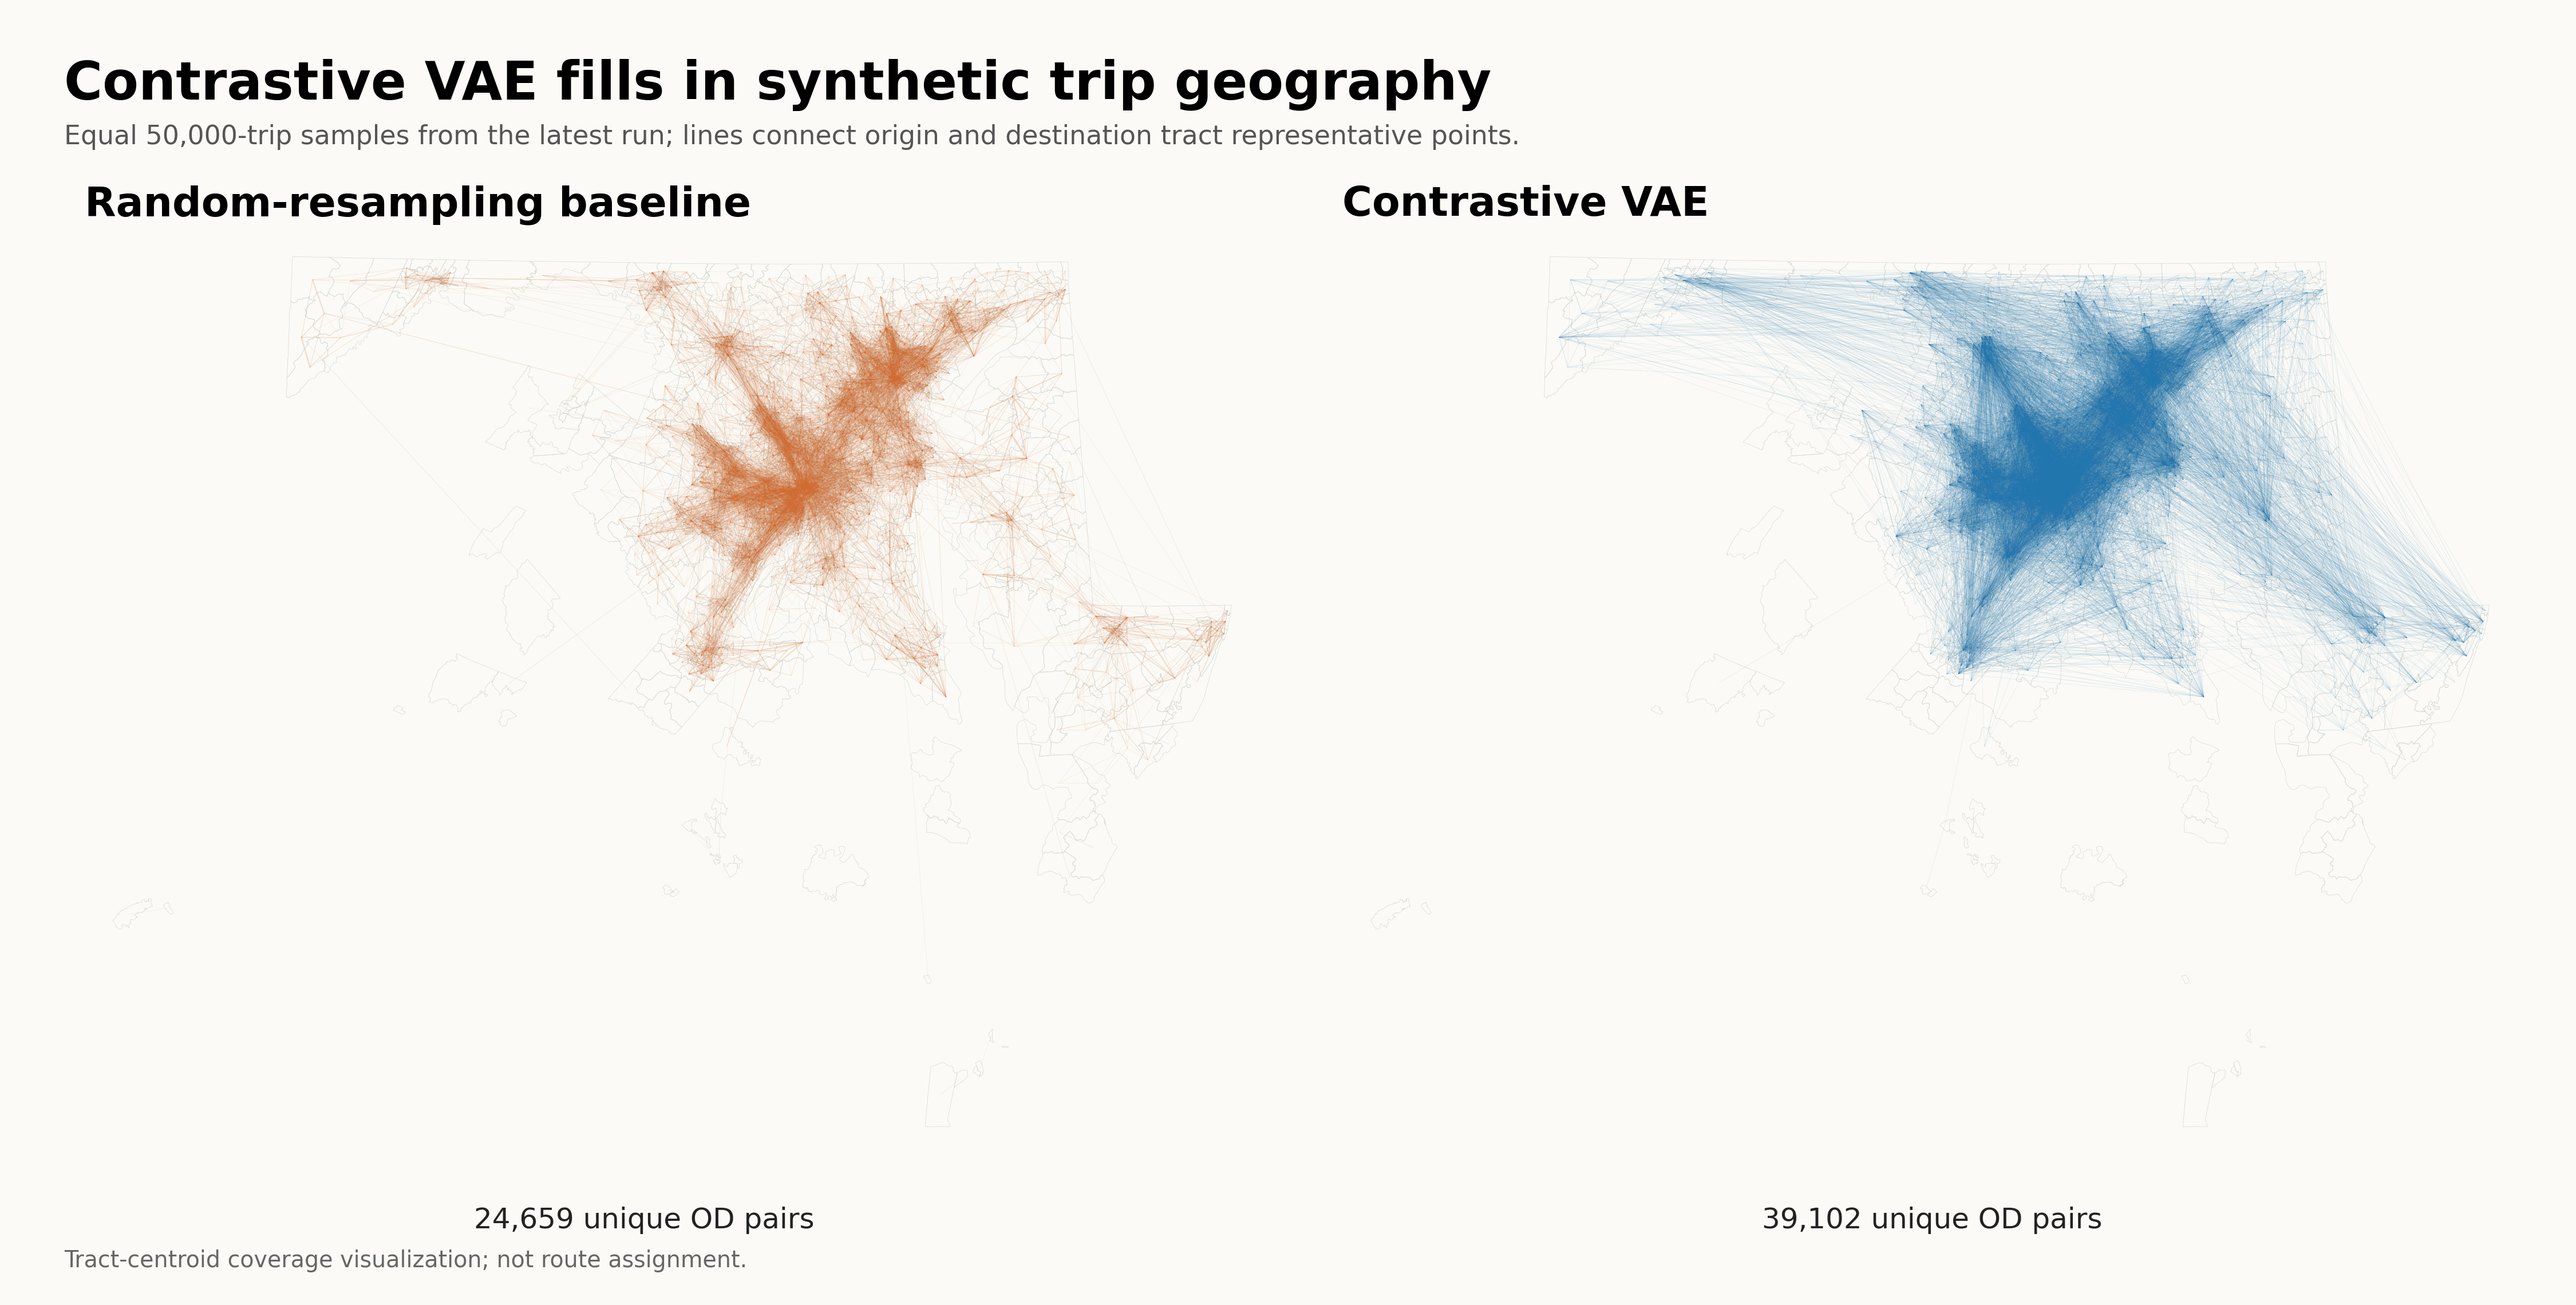
\includegraphics[width=.96\linewidth]{fig_trip_coverage_resampling_vs_cvae.png}
\caption{\textbf{Spatial trip coverage visualization.} Equal-sized samples of weighted-bootstrap and contrastive-VAE trips are drawn as tract-representative-point lines. This figure visualizes OD support, not routed network paths.}
\label{fig:trip-coverage}
\end{figure}

\subsection{Hyperparameter Sweep and Model Selection}
Before the paper-scale run, a 24-trial focused contrastive-VAE sweep tested latent dimension, depth, width decay, KL coefficient, contrastive coefficient, temperature, dropout, learning rate, batch size, and sampling temperature. The trial score combined marginal similarity, cross-marginal similarity, privacy score, invalid-category penalty, and copy-rate penalty. The final paper configuration corresponds to the high-scoring 512-latent, four-layer, width-decay 0.975, $\beta=0.03$, $\lambda=0.25$, $\tau=0.10$, dropout 0.02, learning-rate 0.0005 configuration. This is not an exhaustive global optimization claim; it is a focused model-selection exercise around stable VAE configurations that produced valid synthetic tables.

\begin{figure}[H]
\centering
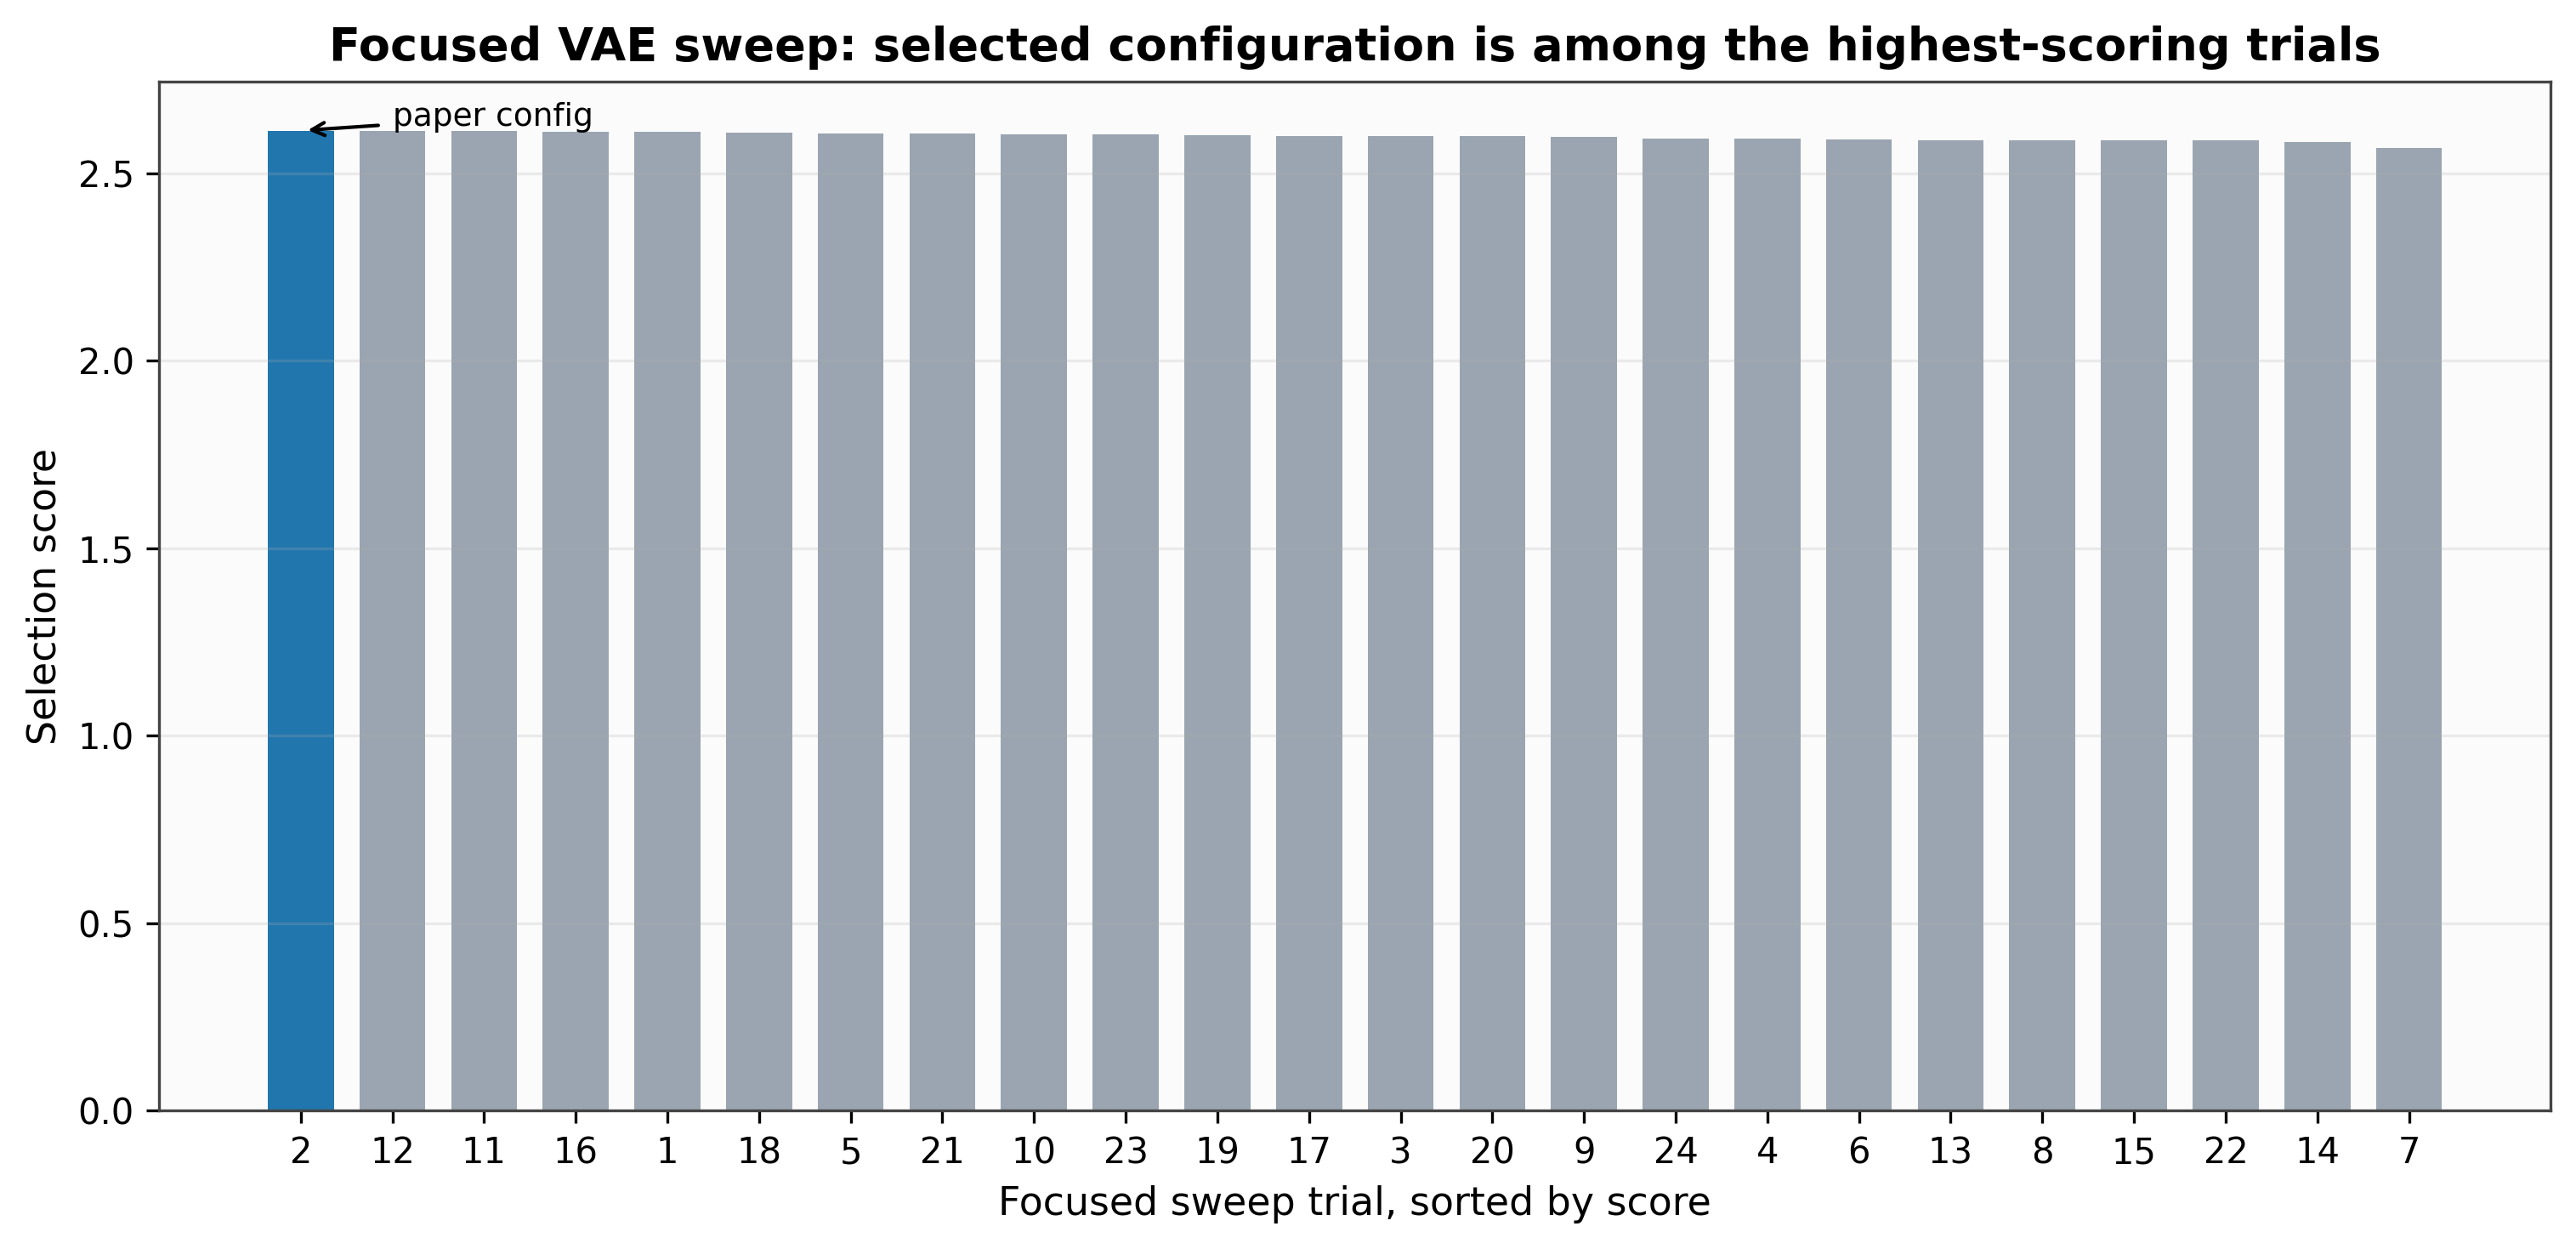
\includegraphics[width=.82\linewidth]{fig_hparam_trial_scores.png}
\caption{\textbf{Focused VAE sweep scores.} The final paper configuration is among the highest-scoring focused sweep trials.}
\label{fig:hparams}
\end{figure}

\subsection{External Annual-Average Screenline Validation}
The annual-average screenline tier compares all four methods across \num{3107} station-mapped screenlines. Table~\ref{tab:annual-results} shows that all methods underpredict screenline traffic on average under the current tract-boundary proxy. The Bayesian network has the lowest annual RMSE and the highest log correlation, while weighted bootstrap has the lowest MAE. The contrastive VAE is not the best global annual method by aggregate error, but it has the largest count of screenlines on which it is the lowest absolute-error method: \num{840} screenlines, compared with \num{817} for the noncontrastive VAE, \num{802} for the Bayesian network, and \num{648} for bootstrap. This combination suggests that the contrastive VAE improves many local OD-crossing patterns but still produces large residuals on enough high-volume screenlines to lose on aggregate annual metrics.

\begin{table}[H]
\centering
\caption{Annual-average MDOT screenline validation. Counts compare synthetic virtual crossings with AAWDT-based station screenline totals.}
\label{tab:annual-results}
\footnotesize
\begin{tabular}{lrrrrrr}
\toprule
\textbf{Method} & \textbf{Screenlines} & \textbf{Pearson log1p} & \textbf{RMSE} & \textbf{MAE} & \textbf{Bias} & \textbf{GEH mean} \\
\midrule
Weighted bootstrap & \num{3107} & 0.2150 & \num{56659} & \num{29855} & \num{-19707} & 208.3 \\
Bayesian network & \num{3107} & 0.2168 & \num{55772} & \num{29918} & \num{-17060} & 207.7 \\
Noncontrastive VAE & \num{3107} & 0.1694 & \num{56145} & \num{30789} & \num{-16083} & 214.1 \\
Contrastive VAE & \num{3107} & 0.1733 & \num{57843} & \num{30572} & \num{-22120} & 215.9 \\
\bottomrule
\end{tabular}
\end{table}

\begin{figure}[H]
\centering
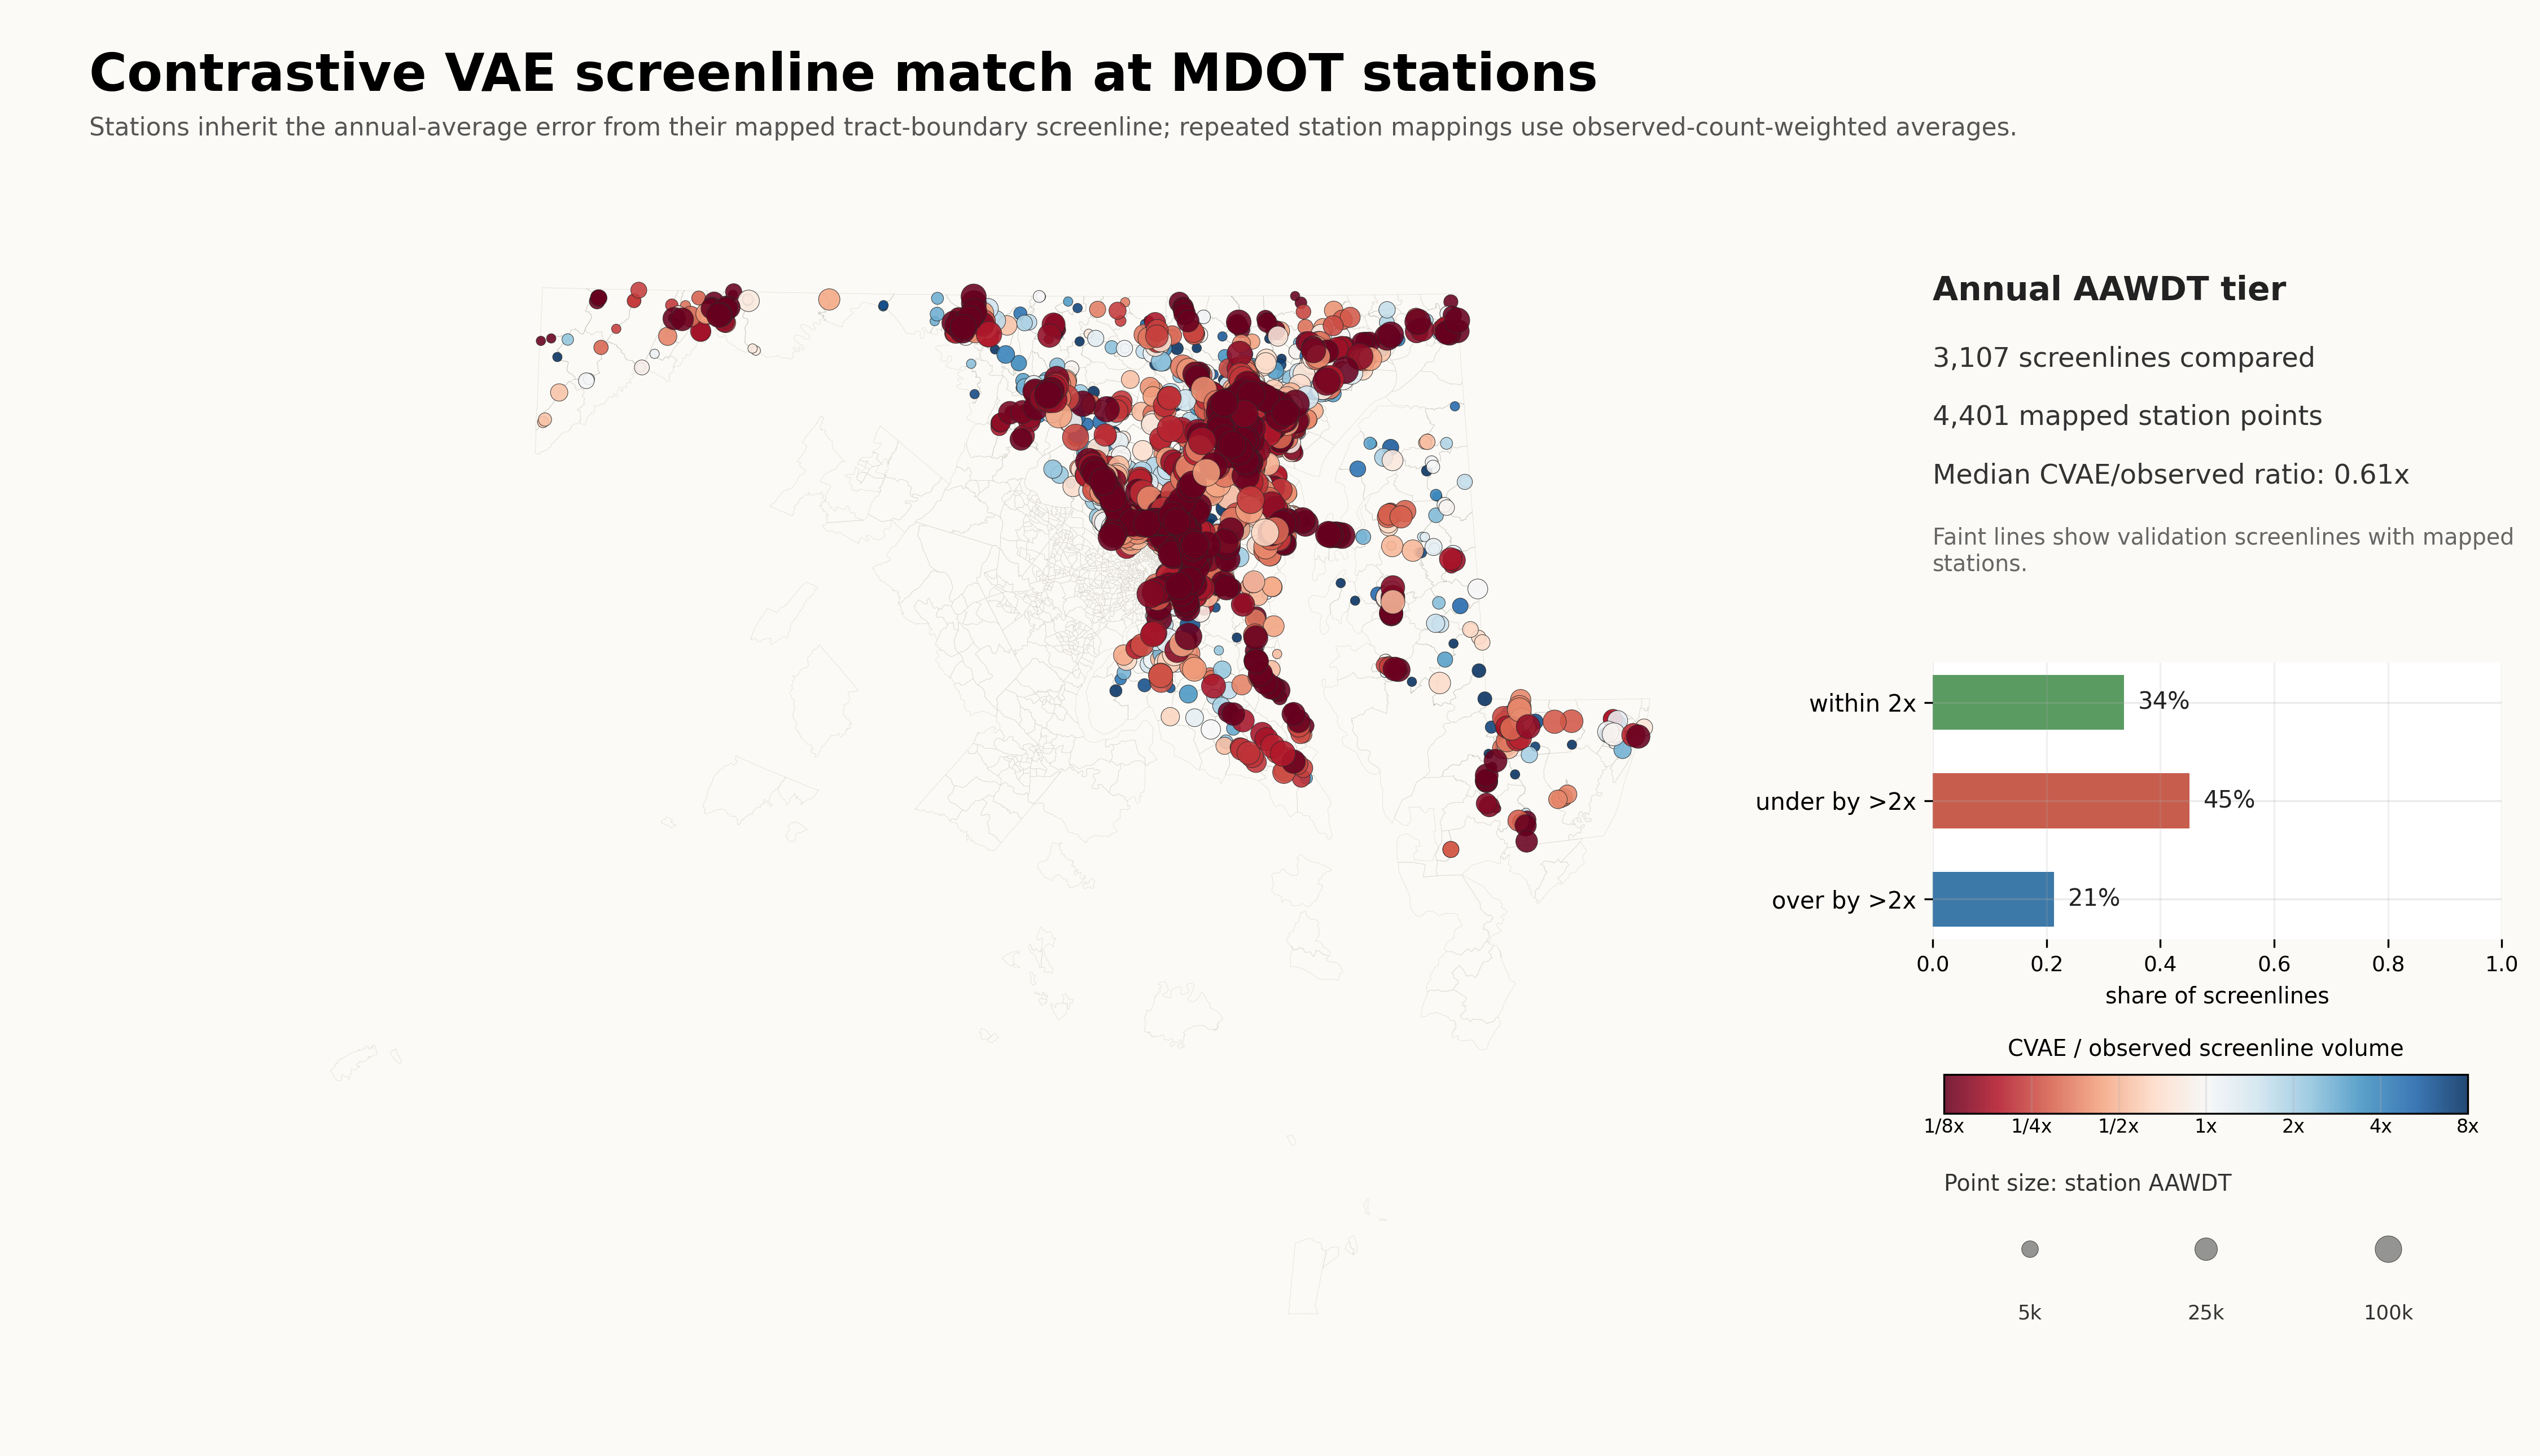
\includegraphics[width=.94\linewidth]{fig_aadt_station_match_map.png}
\caption{\textbf{AADT station-to-screenline validation geography.} MDOT station assignments provide an independent count surface for testing synthetic tract-boundary crossings.}
\label{fig:aadt-map}
\end{figure}

\subsection{External Hourly TMAS Validation}
The hourly tier compares station-hour screenline cells over \num{56} screenlines and method-specific reconstructed-date sets. Here the learned generators substantially outperform weighted bootstrap by RMSE. Weighted bootstrap has hourly RMSE \num{14143}; Bayesian network, noncontrastive VAE, and contrastive VAE reduce this to \num{7169}, \num{6960}, and \num{6944}, respectively. The contrastive VAE has the lowest hourly RMSE, while the noncontrastive VAE has the highest log correlation and lowest MAE. The practical interpretation is that learned generators better distribute hourly screenline demand than direct row resampling, but the two VAE variants remain close and the advantage depends on the metric.

\begin{table}[H]
\centering
\caption{Hourly FHWA TMAS screenline validation. Observed hourly screenline counts are scaled by annual station share of the screenline.}
\label{tab:hourly-results}
\footnotesize
\begin{tabular}{lrrrrrr}
\toprule
\textbf{Method} & \textbf{Cells} & \textbf{Pearson log1p} & \textbf{RMSE} & \textbf{MAE} & \textbf{Bias} & \textbf{GEH mean} \\
\midrule
Weighted bootstrap & \num{537936} & 0.0536 & \num{14143} & \num{5756} & \num{-4266} & 126.0 \\
Bayesian network & \num{624360} & 0.1549 & \num{7169} & \num{4985} & \num{-4064} & 117.9 \\
Noncontrastive VAE & \num{578232} & 0.1750 & \num{6960} & \num{4923} & \num{-4057} & 116.6 \\
Contrastive VAE & \num{601440} & 0.1422 & \num{6944} & \num{4945} & \num{-4288} & 118.2 \\
\bottomrule
\end{tabular}
\end{table}

\begin{figure}[H]
\centering
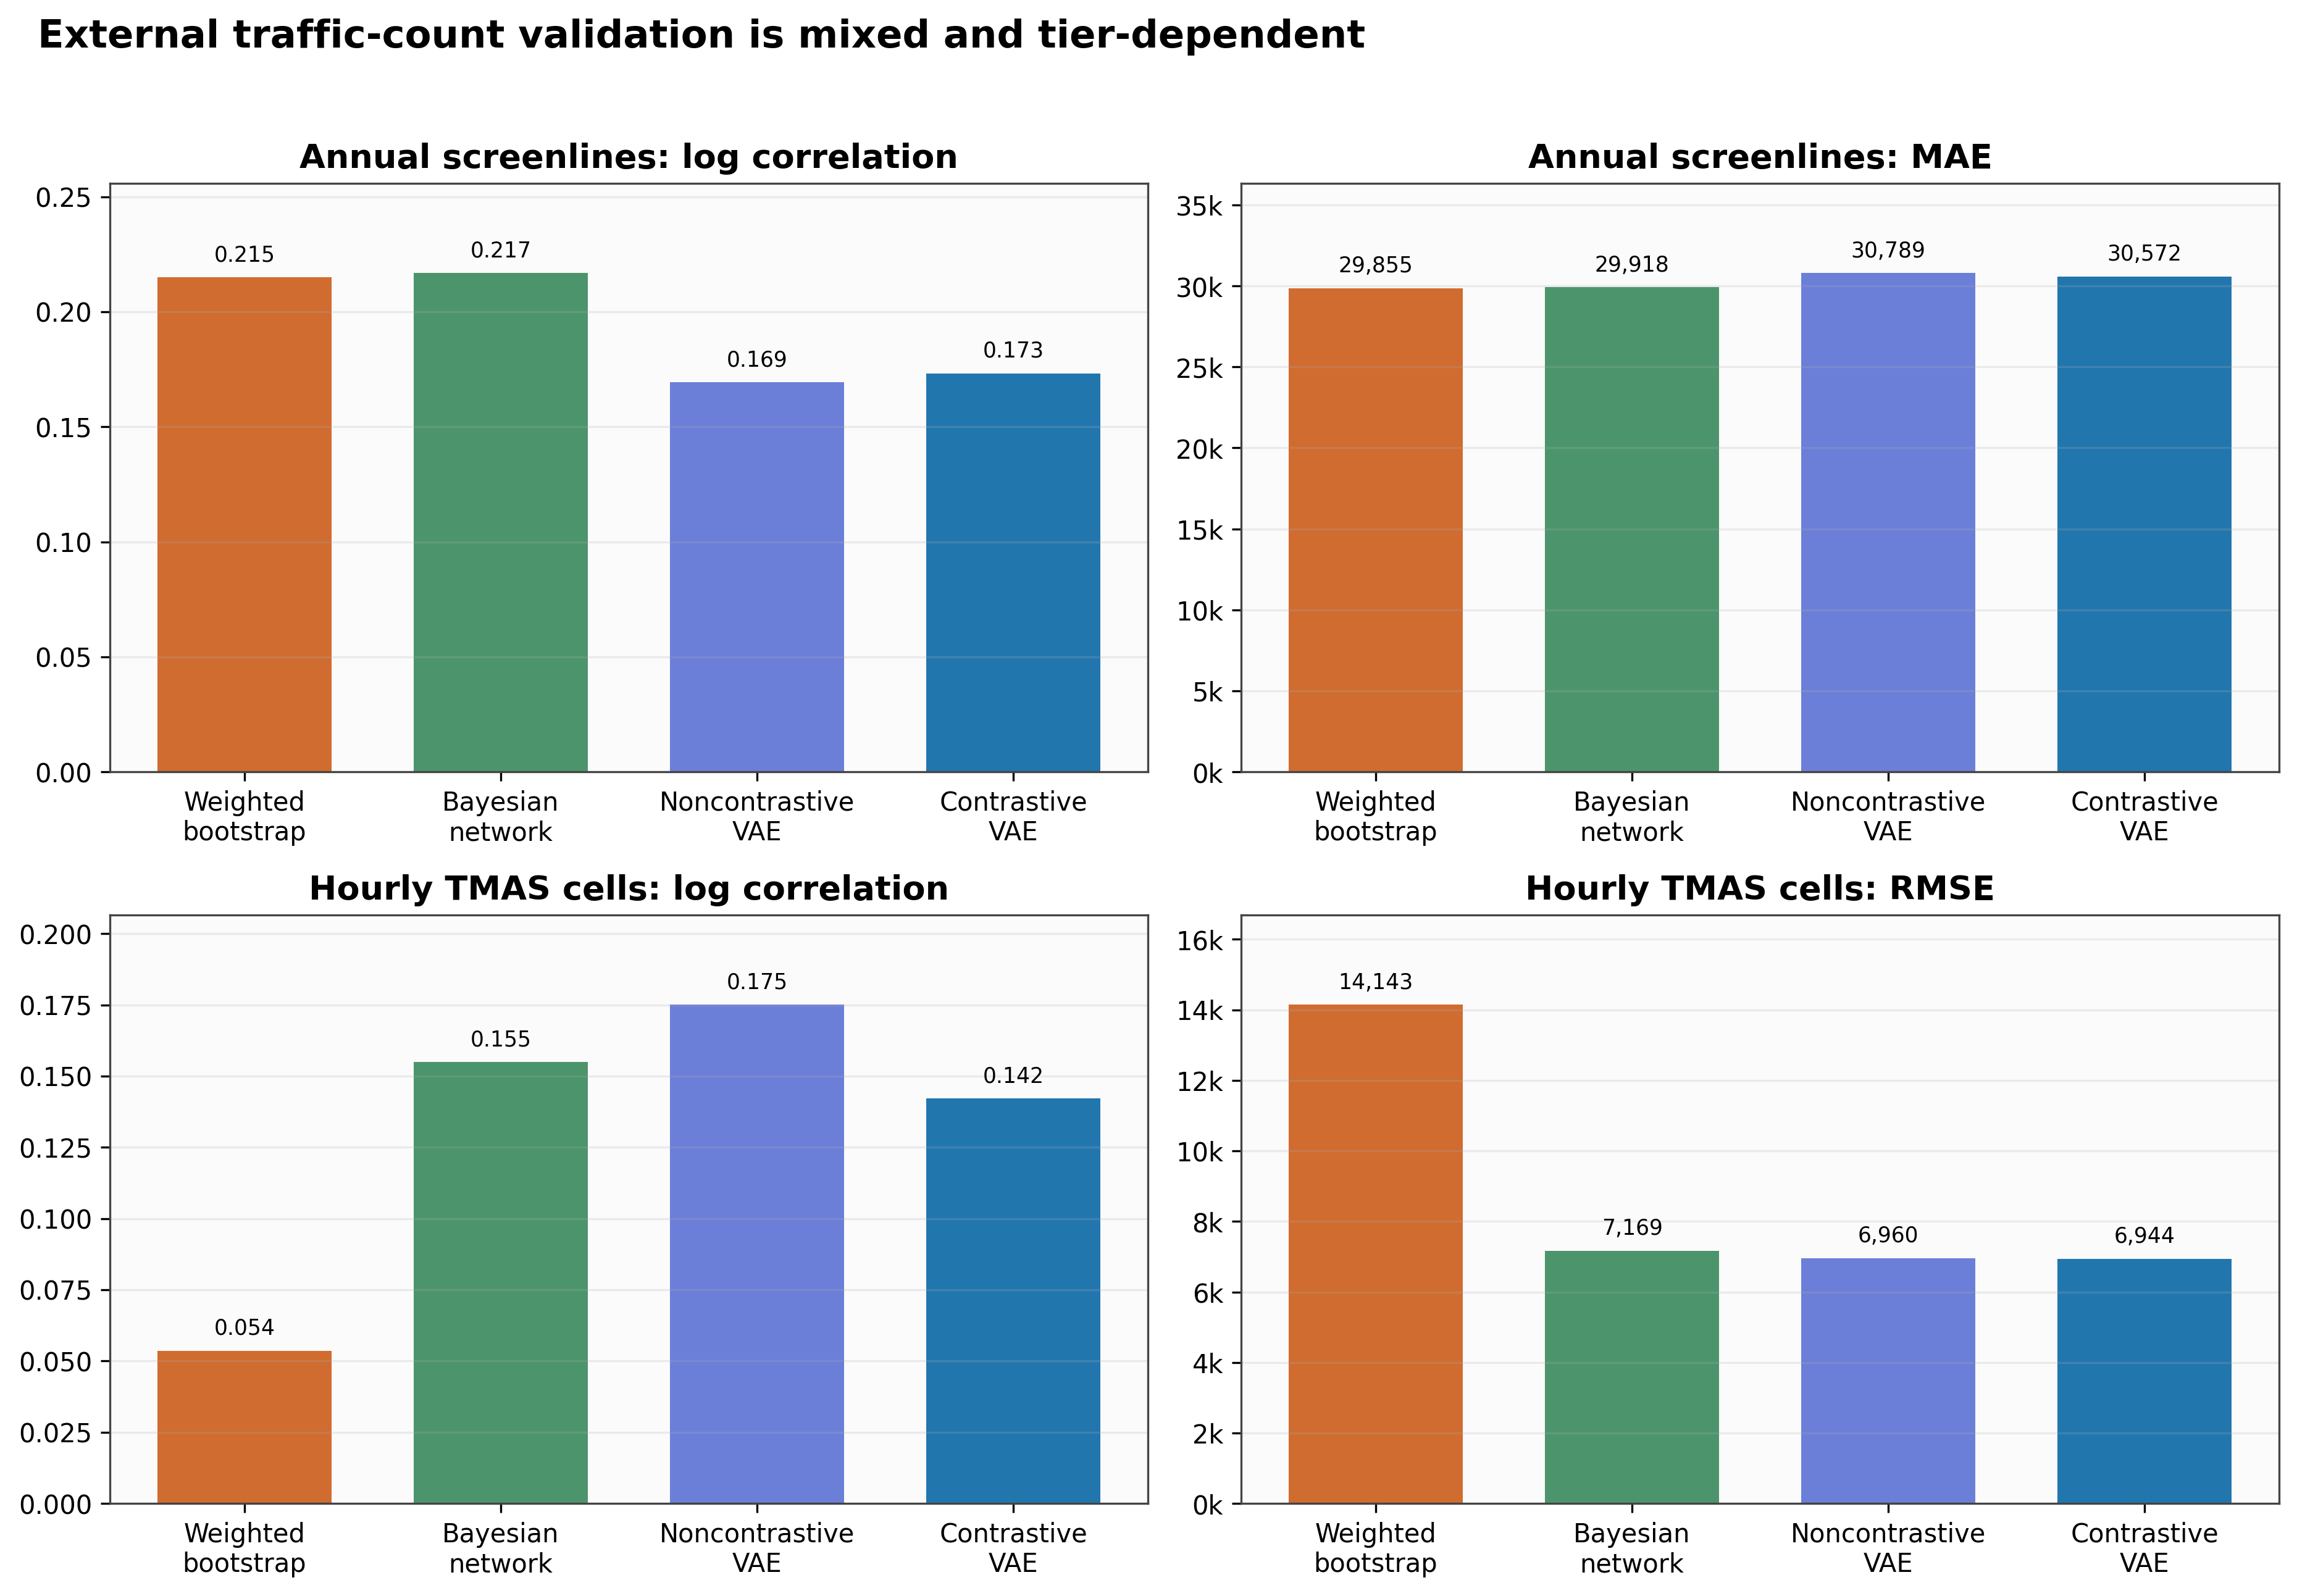
\includegraphics[width=.95\linewidth]{fig_traffic_validation_metrics.png}
\caption{\textbf{External count-validation metrics.} Annual and hourly validation emphasize different properties; the hourly tier favors learned generators over row resampling, while annual totals remain difficult under the current screenline proxy.}
\label{fig:traffic-metrics}
\end{figure}

\begin{figure}[H]
\centering
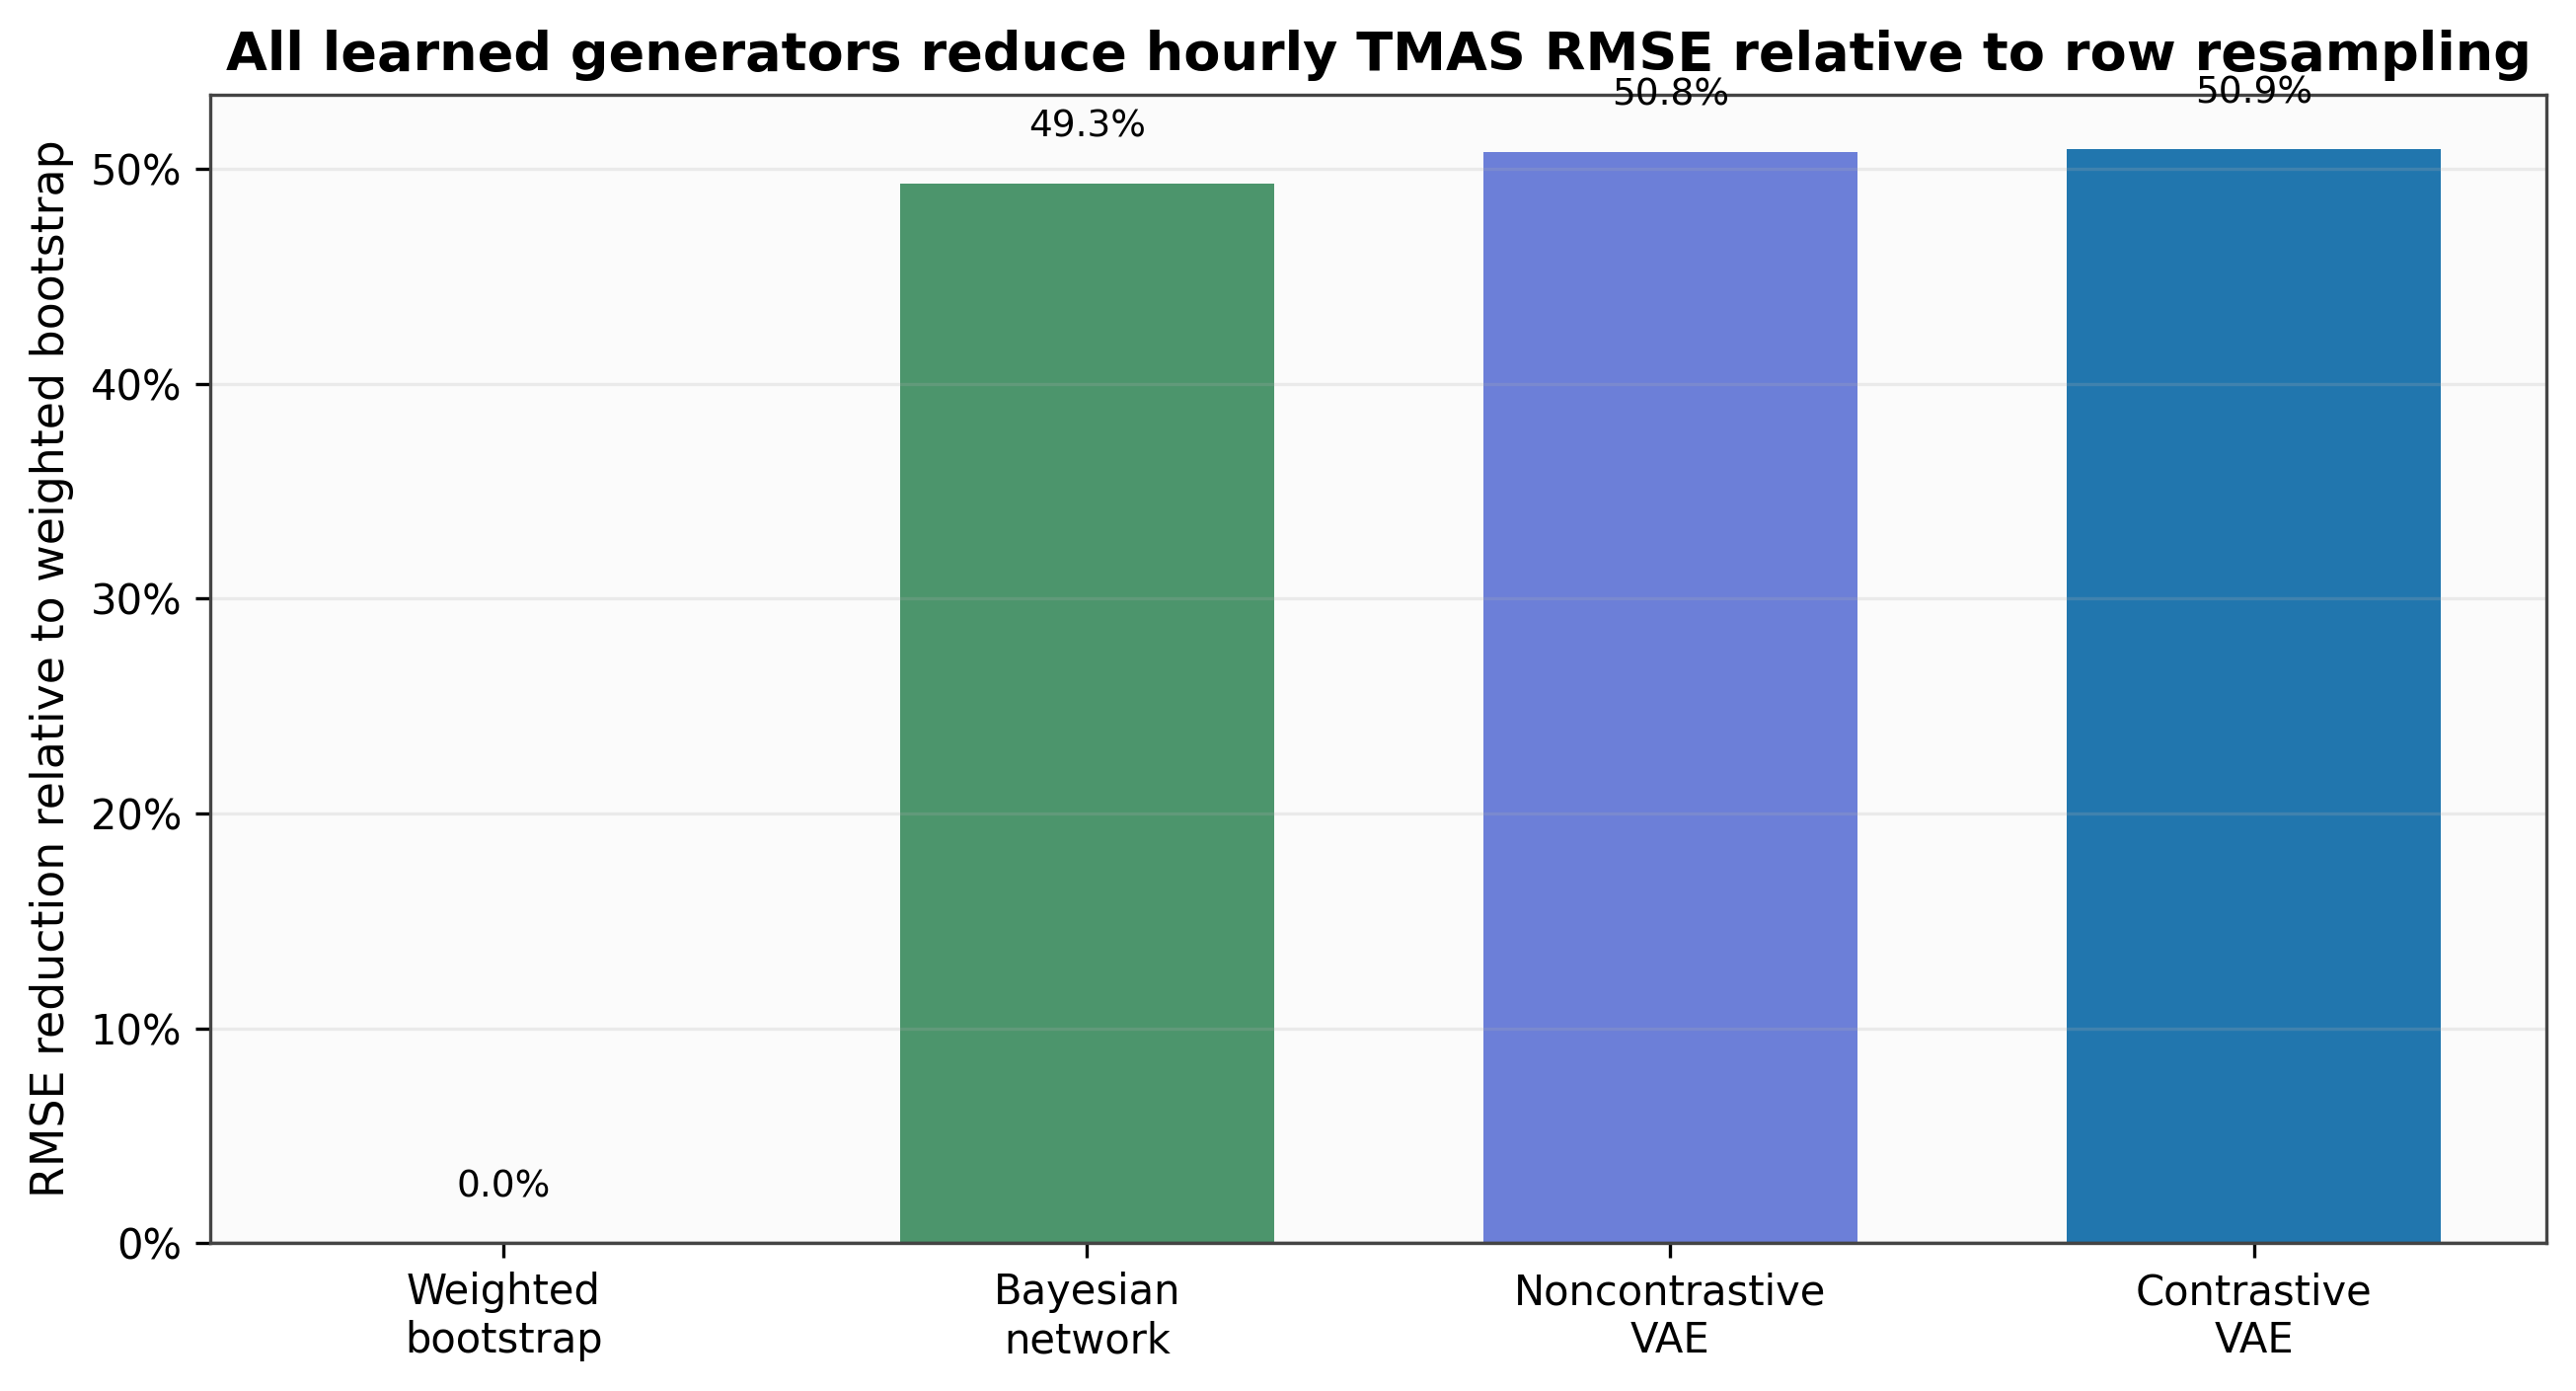
\includegraphics[width=.80\linewidth]{fig_hourly_rmse_reduction.png}
\caption{\textbf{Hourly RMSE reduction relative to weighted bootstrap.} All learned generators reduce hourly TMAS RMSE, with the contrastive VAE obtaining the lowest RMSE in this run.}
\label{fig:hourly-reduction}
\end{figure}

\section{Discussion}\label{sec:discussion}
The central lesson is that ``best'' depends on the property being valued. If the only objective is to reproduce weighted survey marginals, weighted bootstrap is extremely difficult to beat. But that success is achieved by copying the survey. If the objective is non-copying synthetic diversity, the VAEs and Bayesian network are preferable. If the objective is selected behavioral dependence, the contrastive VAE improves the noncontrastive VAE but still trails the Bayesian network and bootstrap on some internal summaries. If the objective is external hourly traffic-count plausibility, all learned generators improve markedly over bootstrap, and the contrastive VAE has the best hourly RMSE. If the objective is annual-average screenline totals, the current proxy remains a hard test for every method.

This pattern is scientifically useful. It prevents a single metric from hiding the generative tradeoff. Copying produces excellent internal fidelity but poor privacy and diversity. A tree-structured Bayesian network preserves many simple distributions but has limited higher-order expressiveness. A VAE can generate much broader OD support, but broader support can harm marginal and annual-count accuracy if not constrained by external controls. Contrastive regularization helps the VAE recover some joint structure, especially cross-marginal trip relationships, but it does not eliminate the need for better spatial constraints or route-aware validation.

The screenline validation should also be read carefully. The method does not assign trips to a road network. It draws centroid-to-centroid tract lines, records tract-boundary crossings, maps nearby MDOT stations to tract boundaries, and compares virtual crossings with annual or hourly count summaries. This is valuable because it is independent of the survey and transparent enough to audit, but it is still a proxy. Large annual errors may reflect synthetic demand, station-to-boundary assignment, tract representative points, screenline coverage, average-day scaling, or the fact that observed station counts measure road facilities while synthetic crossings measure tract-boundary movements. These limitations are precisely why external validation belongs in the workflow: it reveals where a model that is internally plausible is not yet a calibrated traffic-demand model.

\section{Limitations and Future Work}\label{sec:limitations}
First, the experiment is trip-level rather than household-plan-level. It preserves many household and person attributes within trip records, but it does not enforce household consistency across multiple trips. Second, the one-million-row cap requires sample expansion for traffic-count validation. This keeps experiments tractable but introduces scaling assumptions, especially when date strata are expanded to average-day counts. Third, the privacy diagnostics are not formal privacy guarantees; differential privacy would require a different training mechanism and privacy accounting. Fourth, the external screenline method is Maryland-centered because the dense annual station layer is MDOT SHA AADT/AAWDT. Virginia and DC annual traffic-volume layers were identified as future extensions, but the current two-prong validation uses MDOT annual counts and FHWA TMAS hourly stations. Fifth, centroid-line tract crossing is a deliberately simple proxy and should be replaced or complemented by network route assignment when the research question shifts from trip synthesis to link-volume calibration.

Future work should condition generation on known external controls, enforce household-plan coherence, add feasibility constraints for structural-zero prevention, evaluate route-assigned link counts and speeds, and test conditional synthesis scenarios such as policy-specific OD, mode, or time-of-day perturbations. A particularly promising direction is to combine contrastive tabular representation learning with explicit spatial priors so that novel OD support is generated where it is demographically and geographically credible.

\section{Conclusion}\label{sec:conclusion}
This paper presents a reproducible contrastive VAE experiment for generating population-scale synthetic trip records from travel surveys. The implemented run uses survey weights as expansion and training weights, excludes weights from generated records, compares against weighted bootstrap, Bayesian network, and noncontrastive VAE baselines, and validates results through internal marginals, cross-marginals, copying diagnostics, OD support, and independent traffic-count screenlines.

The findings are not a simple victory lap for one model. They are a map of tradeoffs. Bootstrap remains the internal distributional upper bound but copies records. The Bayesian network is strong on one-way distributions but less expressive for selected dependencies. The contrastive VAE generates broad novel OD support with zero exact-copy rate and improves cross-marginal structure relative to the noncontrastive VAE. External validation shows that learned generators improve hourly count plausibility relative to bootstrap, while annual screenline totals remain challenging. The contribution is therefore a rigorous synthesis-and-validation framework for advancing contrastive VAE-generated trip data from travel surveys toward credible agent-based demand inputs.

\section*{Acknowledgements}
This manuscript was prepared from the reproducible experiment artifacts in \texttt{paper\_wctr\_1m\_vae\_sweep}. Any remaining interpretation errors are the responsibility of the authors.

\bibliographystyle{elsarticle-num}
\bibliography{references}

\end{document}
